\documentclass[aspectratio=169,11pt]{beamer}
% ==========================================================================
%  KSA lecture-slide theme  =  stock beamer "Boadilla"  +  KSA colour theme
%  brand colours sampled from the official KSA symbol mark:
%    Deep Prussian Blue  #2E3192   (지성 - intellect)
%    Golden Gray         #D6CBB1   (감성 - sensibility)
%  Engine: XeLaTeX.  Usage:
%    \documentclass[aspectratio=169,11pt]{beamer}
%    % ==========================================================================
%  KSA lecture-slide theme  =  stock beamer "Boadilla"  +  KSA colour theme
%  brand colours sampled from the official KSA symbol mark:
%    Deep Prussian Blue  #2E3192   (지성 - intellect)
%    Golden Gray         #D6CBB1   (감성 - sensibility)
%  Engine: XeLaTeX.  Usage:
%    \documentclass[aspectratio=169,11pt]{beamer}
%    % ==========================================================================
%  KSA lecture-slide theme  =  stock beamer "Boadilla"  +  KSA colour theme
%  brand colours sampled from the official KSA symbol mark:
%    Deep Prussian Blue  #2E3192   (지성 - intellect)
%    Golden Gray         #D6CBB1   (감성 - sensibility)
%  Engine: XeLaTeX.  Usage:
%    \documentclass[aspectratio=169,11pt]{beamer}
%    \input{../theme/ksa-theme.tex}
% ==========================================================================

\usepackage{fontspec}
\usepackage{amsmath,amssymb}
\usepackage{graphicx}
\graphicspath{{figs/}{../figs/}}
\usepackage{booktabs}
\usepackage{listings}

% ---- fonts (no ctex/xeCJK on this box -> fontspec drives CJK directly) -----
\defaultfontfeatures{Ligatures=TeX}
\setmainfont{Noto Sans CJK KR}
\setsansfont{Noto Sans CJK KR}
\setmonofont{Noto Sans Mono CJK KR}[Scale=0.92]

% ---- base theme: stock Boadilla ------------------------------------------
\usetheme{Boadilla}
\usefonttheme{professionalfonts}
\setbeamertemplate{navigation symbols}{}

% ---- KSA colour theme (recolour the stock theme) --------------------------
\definecolor{ksablue}{HTML}{2E3192}
\definecolor{ksabluedk}{HTML}{20226A}
\definecolor{ksagold}{HTML}{D6CBB1}
\definecolor{ksagolddk}{HTML}{A9976B}
\definecolor{ksared}{HTML}{C0392B}
\definecolor{ksagray}{HTML}{5B5B5B}

\setbeamercolor{structure}{fg=ksablue}
\setbeamercolor{alerted text}{fg=ksared}

\setbeamercolor{palette primary}{fg=white,           bg=ksablue}
\setbeamercolor{palette secondary}{fg=white,         bg=ksablue!85!black}
\setbeamercolor{palette tertiary}{fg=white,          bg=ksabluedk}
\setbeamercolor{titlelike}{fg=ksablue}
\setbeamercolor{frametitle}{fg=ksablue,bg=}
\setbeamercolor{title}{fg=ksablue}
\setbeamercolor{author}{fg=ksagray}
\setbeamercolor{institute}{fg=ksagray}
\setbeamercolor{block title}{fg=white,bg=ksablue}
\setbeamercolor{block body}{fg=black!85,bg=ksablue!6}
\setbeamercolor{item}{fg=ksablue}
\setbeamercolor{section in toc}{fg=black!85}

\setbeamerfont{frametitle}{series=\bfseries}
\setbeamerfont{title}{series=\bfseries}

% ---- footline:  KSA mark | "Made by ..." | n / N   (matches reference) ----
\newcommand{\ksacredit}{Made by Sumin Han \,\textperiodcentered\, suminhan@ksa.hs.kr}
\setbeamertemplate{footline}{%
  \hbox{%
    \begin{beamercolorbox}[wd=.18\paperwidth,ht=2.6ex,dp=1.5ex,leftskip=1.1em]{}%
      \raisebox{-0.35ex}{
\includegraphics[height=2.0ex]{ksa-logo.png}}%
    \end{beamercolorbox}%
    \begin{beamercolorbox}[wd=.64\paperwidth,ht=2.6ex,dp=1.5ex,center]{}%
      {\scriptsize\color{ksagray}\ksacredit}%
    \end{beamercolorbox}%
    \begin{beamercolorbox}[wd=.18\paperwidth,ht=2.6ex,dp=1.5ex,rightskip=1.1em]{}%
      \hfill{\scriptsize\color{ksablue}\insertframenumber\,/\,\inserttotalframenumber}%
    \end{beamercolorbox}%
  }%
  \vskip2pt
}

% ---- section divider: stock \sectionpage, KSA-coloured -------------------
\setbeamertemplate{section page}{%
  \begingroup\centering
    {\color{ksagolddk}\rule{0.16\paperwidth}{1pt}}\par\vskip1.0em
    {\usebeamerfont{title}\color{ksablue}\insertsectionhead\par}\vskip1.0em
    {\color{ksagolddk}\rule{0.16\paperwidth}{1pt}}\par
  \endgroup
}
\AtBeginSection[]{\begin{frame}[plain,noframenumbering]\vfill\sectionpage\vfill\end{frame}}

% ---- code listings ------------------------------------------------------------
\lstdefinestyle{ksa}{%
  basicstyle=\ttfamily\scriptsize,
  keywordstyle=\color{ksablue}\bfseries,
  commentstyle=\color{ksagray}\itshape,
  stringstyle=\color{ksagolddk},
  numberstyle=\tiny\color{ksagray},
  backgroundcolor=\color{ksablue!6},
  frame=leftline, framerule=1.4pt, rulecolor=\color{ksablue},
  xleftmargin=1em, aboveskip=0.8em, belowskip=0.4em,
  showstringspaces=false, breaklines=true, language=Python,
}
\lstset{style=ksa}

% ---- handy macros -----------------------------------------------------------
\newcommand{\kb}[1]{\textbf{\color{ksablue}#1}}   % blue keyword
\newcommand{\kq}[1]{\textbf{\color{ksared}#1}}    % red key-question

% ==========================================================================

\usepackage{fontspec}
\usepackage{amsmath,amssymb}
\usepackage{graphicx}
\graphicspath{{figs/}{../figs/}}
\usepackage{booktabs}
\usepackage{listings}

% ---- fonts (no ctex/xeCJK on this box -> fontspec drives CJK directly) -----
\defaultfontfeatures{Ligatures=TeX}
\setmainfont{Noto Sans CJK KR}
\setsansfont{Noto Sans CJK KR}
\setmonofont{Noto Sans Mono CJK KR}[Scale=0.92]

% ---- base theme: stock Boadilla ------------------------------------------
\usetheme{Boadilla}
\usefonttheme{professionalfonts}
\setbeamertemplate{navigation symbols}{}

% ---- KSA colour theme (recolour the stock theme) --------------------------
\definecolor{ksablue}{HTML}{2E3192}
\definecolor{ksabluedk}{HTML}{20226A}
\definecolor{ksagold}{HTML}{D6CBB1}
\definecolor{ksagolddk}{HTML}{A9976B}
\definecolor{ksared}{HTML}{C0392B}
\definecolor{ksagray}{HTML}{5B5B5B}

\setbeamercolor{structure}{fg=ksablue}
\setbeamercolor{alerted text}{fg=ksared}

\setbeamercolor{palette primary}{fg=white,           bg=ksablue}
\setbeamercolor{palette secondary}{fg=white,         bg=ksablue!85!black}
\setbeamercolor{palette tertiary}{fg=white,          bg=ksabluedk}
\setbeamercolor{titlelike}{fg=ksablue}
\setbeamercolor{frametitle}{fg=ksablue,bg=}
\setbeamercolor{title}{fg=ksablue}
\setbeamercolor{author}{fg=ksagray}
\setbeamercolor{institute}{fg=ksagray}
\setbeamercolor{block title}{fg=white,bg=ksablue}
\setbeamercolor{block body}{fg=black!85,bg=ksablue!6}
\setbeamercolor{item}{fg=ksablue}
\setbeamercolor{section in toc}{fg=black!85}

\setbeamerfont{frametitle}{series=\bfseries}
\setbeamerfont{title}{series=\bfseries}

% ---- footline:  KSA mark | "Made by ..." | n / N   (matches reference) ----
\newcommand{\ksacredit}{Made by Sumin Han \,\textperiodcentered\, suminhan@ksa.hs.kr}
\setbeamertemplate{footline}{%
  \hbox{%
    \begin{beamercolorbox}[wd=.18\paperwidth,ht=2.6ex,dp=1.5ex,leftskip=1.1em]{}%
      \raisebox{-0.35ex}{
\includegraphics[height=2.0ex]{ksa-logo.png}}%
    \end{beamercolorbox}%
    \begin{beamercolorbox}[wd=.64\paperwidth,ht=2.6ex,dp=1.5ex,center]{}%
      {\scriptsize\color{ksagray}\ksacredit}%
    \end{beamercolorbox}%
    \begin{beamercolorbox}[wd=.18\paperwidth,ht=2.6ex,dp=1.5ex,rightskip=1.1em]{}%
      \hfill{\scriptsize\color{ksablue}\insertframenumber\,/\,\inserttotalframenumber}%
    \end{beamercolorbox}%
  }%
  \vskip2pt
}

% ---- section divider: stock \sectionpage, KSA-coloured -------------------
\setbeamertemplate{section page}{%
  \begingroup\centering
    {\color{ksagolddk}\rule{0.16\paperwidth}{1pt}}\par\vskip1.0em
    {\usebeamerfont{title}\color{ksablue}\insertsectionhead\par}\vskip1.0em
    {\color{ksagolddk}\rule{0.16\paperwidth}{1pt}}\par
  \endgroup
}
\AtBeginSection[]{\begin{frame}[plain,noframenumbering]\vfill\sectionpage\vfill\end{frame}}

% ---- code listings ------------------------------------------------------------
\lstdefinestyle{ksa}{%
  basicstyle=\ttfamily\scriptsize,
  keywordstyle=\color{ksablue}\bfseries,
  commentstyle=\color{ksagray}\itshape,
  stringstyle=\color{ksagolddk},
  numberstyle=\tiny\color{ksagray},
  backgroundcolor=\color{ksablue!6},
  frame=leftline, framerule=1.4pt, rulecolor=\color{ksablue},
  xleftmargin=1em, aboveskip=0.8em, belowskip=0.4em,
  showstringspaces=false, breaklines=true, language=Python,
}
\lstset{style=ksa}

% ---- handy macros -----------------------------------------------------------
\newcommand{\kb}[1]{\textbf{\color{ksablue}#1}}   % blue keyword
\newcommand{\kq}[1]{\textbf{\color{ksared}#1}}    % red key-question

% ==========================================================================

\usepackage{fontspec}
\usepackage{amsmath,amssymb}
\usepackage{graphicx}
\graphicspath{{figs/}{../figs/}}
\usepackage{booktabs}
\usepackage{listings}

% ---- fonts (no ctex/xeCJK on this box -> fontspec drives CJK directly) -----
\defaultfontfeatures{Ligatures=TeX}
\setmainfont{Noto Sans CJK KR}
\setsansfont{Noto Sans CJK KR}
\setmonofont{Noto Sans Mono CJK KR}[Scale=0.92]

% ---- base theme: stock Boadilla ------------------------------------------
\usetheme{Boadilla}
\usefonttheme{professionalfonts}
\setbeamertemplate{navigation symbols}{}

% ---- KSA colour theme (recolour the stock theme) --------------------------
\definecolor{ksablue}{HTML}{2E3192}
\definecolor{ksabluedk}{HTML}{20226A}
\definecolor{ksagold}{HTML}{D6CBB1}
\definecolor{ksagolddk}{HTML}{A9976B}
\definecolor{ksared}{HTML}{C0392B}
\definecolor{ksagray}{HTML}{5B5B5B}

\setbeamercolor{structure}{fg=ksablue}
\setbeamercolor{alerted text}{fg=ksared}

\setbeamercolor{palette primary}{fg=white,           bg=ksablue}
\setbeamercolor{palette secondary}{fg=white,         bg=ksablue!85!black}
\setbeamercolor{palette tertiary}{fg=white,          bg=ksabluedk}
\setbeamercolor{titlelike}{fg=ksablue}
\setbeamercolor{frametitle}{fg=ksablue,bg=}
\setbeamercolor{title}{fg=ksablue}
\setbeamercolor{author}{fg=ksagray}
\setbeamercolor{institute}{fg=ksagray}
\setbeamercolor{block title}{fg=white,bg=ksablue}
\setbeamercolor{block body}{fg=black!85,bg=ksablue!6}
\setbeamercolor{item}{fg=ksablue}
\setbeamercolor{section in toc}{fg=black!85}

\setbeamerfont{frametitle}{series=\bfseries}
\setbeamerfont{title}{series=\bfseries}

% ---- footline:  KSA mark | "Made by ..." | n / N   (matches reference) ----
\newcommand{\ksacredit}{Made by Sumin Han \,\textperiodcentered\, suminhan@ksa.hs.kr}
\setbeamertemplate{footline}{%
  \hbox{%
    \begin{beamercolorbox}[wd=.18\paperwidth,ht=2.6ex,dp=1.5ex,leftskip=1.1em]{}%
      \raisebox{-0.35ex}{
\includegraphics[height=2.0ex]{ksa-logo.png}}%
    \end{beamercolorbox}%
    \begin{beamercolorbox}[wd=.64\paperwidth,ht=2.6ex,dp=1.5ex,center]{}%
      {\scriptsize\color{ksagray}\ksacredit}%
    \end{beamercolorbox}%
    \begin{beamercolorbox}[wd=.18\paperwidth,ht=2.6ex,dp=1.5ex,rightskip=1.1em]{}%
      \hfill{\scriptsize\color{ksablue}\insertframenumber\,/\,\inserttotalframenumber}%
    \end{beamercolorbox}%
  }%
  \vskip2pt
}

% ---- section divider: stock \sectionpage, KSA-coloured -------------------
\setbeamertemplate{section page}{%
  \begingroup\centering
    {\color{ksagolddk}\rule{0.16\paperwidth}{1pt}}\par\vskip1.0em
    {\usebeamerfont{title}\color{ksablue}\insertsectionhead\par}\vskip1.0em
    {\color{ksagolddk}\rule{0.16\paperwidth}{1pt}}\par
  \endgroup
}
\AtBeginSection[]{\begin{frame}[plain,noframenumbering]\vfill\sectionpage\vfill\end{frame}}

% ---- code listings ------------------------------------------------------------
\lstdefinestyle{ksa}{%
  basicstyle=\ttfamily\scriptsize,
  keywordstyle=\color{ksablue}\bfseries,
  commentstyle=\color{ksagray}\itshape,
  stringstyle=\color{ksagolddk},
  numberstyle=\tiny\color{ksagray},
  backgroundcolor=\color{ksablue!6},
  frame=leftline, framerule=1.4pt, rulecolor=\color{ksablue},
  xleftmargin=1em, aboveskip=0.8em, belowskip=0.4em,
  showstringspaces=false, breaklines=true, language=Python,
}
\lstset{style=ksa}

% ---- handy macros -----------------------------------------------------------
\newcommand{\kb}[1]{\textbf{\color{ksablue}#1}}   % blue keyword
\newcommand{\kq}[1]{\textbf{\color{ksared}#1}}    % red key-question


\title{거리 기반 모델과 클러스터링: kNN, k-means, GMM/EM}
\subtitle{kNN과 편향-분산 · 차원의 저주와 k 튜닝 · k-means · GMM과 EM/LDA}
\author{Machine Learning 1 \,\textperiodcentered\, 4주차}
\institute{한국과학영재학교 (KSA)}
\date{Chapter 4}

\begin{document}
\begin{frame}[plain,noframenumbering]\titlepage\end{frame}

\begin{frame}{이번 주차 개요}
  ``당신은 가장 가까운 다섯 친구의 평균이다'' --- 이 한 줄이
  \kb{k-최근접이웃(kNN)}의 알고리즘 그 자체다. 거리를 직접 재는
  세 주인공: kNN(지도) · k-means(비지도) · GMM/EM(확률적 일반화).
  \vskip0.8em
  \begin{columns}[T]
    \begin{column}{0.55\textwidth}
      \textbf{이 챕터를 마치면}
      \begin{itemize}\small
        \item kNN이 게으른(lazy)·비모수 방법임을, $k$를 키우며
          결정경계가 톱니바퀴 $\to$ 직선으로 변하는 과정을
          \kb{편향-분산 트레이드오프}로 설명
        \item 차원의 저주를 부피 공식 $p^{1/n}$과 이웃 간 거리 스케일로
          \textbf{정량적으로} 설명, 검증셋으로 $k$ 튜닝 코드 작성
        \item k-means 반복이 SSE를 단조감소시켜 수렴함을 수학으로 보임
        \item GMM이 왜 MLE로 바로 풀리지 않는지(우도가 \textbf{곱의
          합}), EM 한 라운드를 손계산
        \item 옌센 부등식 4줄로 ``우도가 절대 줄지 않는다'' 증명,
          $K$는 \kb{BIC}로 고르고 \kb{LDA}와 대비
      \end{itemize}
    \end{column}
    \begin{column}{0.43\textwidth}
      \textbf{네 차시 한 줄}
      \begin{itemize}\small
        \item \kb{4.1} 게으른 학습 · 거리함수·정규화 · 편향-분산
        \item \kb{4.2} 차원의 저주($p^{1/n}$, 동거리) · $k$ 튜닝 실습
        \item \kb{4.3} 수렴 증명 · 엘보우 · k-means++ · 구조적 한계
        \item \kb{4.4} GMM · EM · 옌센 부등식 · BIC · LDA
      \end{itemize}
      \vskip0.6em
      Ch.\,3(생성 모델)이 회피한 \textbf{차원의 저주}를 이번 장은
      정면으로 맞는다. Ch.\,5(SVM)로 가는 다리도 여기서 놓인다.
    \end{column}
  \end{columns}
\end{frame}

% ============================================================
\section{4.1 kNN: 알고리즘, 거리함수, 편향-분산 트레이드오프}

\begin{frame}{``가장 가까운 5명의 평균''}
  \begin{itemize}
    \item 새 데이터를 분류하려면 \textbf{학습도 모델도 없이}:
      가장 가까운 $k$개의 기존 데이터가 뭐라고 답했는지 보고
      다수결로 따른다
    \item 이 단순한 한 줄이 kNN이다 --- 거리를 \textbf{재는 데서
      출발}한다는 공통점이 k-means와 한 장에 묶는 이유
  \end{itemize}
  \vskip0.8em
  \begin{block}{kNN의 성격}
    \kb{게으른(lazy)}: 예측 시점에 거리를 재는 순간 모델이 완성된다 \\
    \kb{비모수(nonparametric)}: 파라미터 없이 점과 점을 비교
  \end{block}
  \kq{새 점의 정답은 ``그 점과 가까운 점들의 정답 평균''일까?}
\end{frame}

\begin{frame}{학습이 없는 학습 알고리즘}
  \begin{columns}[T]
    \begin{column}{0.5\textwidth}
      \textbf{선형/로지스틱 회귀}
      \begin{itemize}\small
        \item 데이터를 보고 파라미터 $w$를 최적화하는
          \kb{학습 단계}가 있음
        \item 학습이 끝나면 $w$만 있으면
          원본 데이터 불필요
      \end{itemize}
      \vskip0.6em
      \textbf{kNN}
      \begin{itemize}\small
        \item ``학습''은 데이터를 \textbf{그냥 저장}해 두는 것뿐
        \item 모든 계산은 \textbf{예측 시점}에: 새 점이 들어오면
          그때서야 모든 점까지 거리를 재고 가까운 점 찾기
      \end{itemize}
    \end{column}
    \begin{column}{0.48\textwidth}
      \begin{block}{장점 --- 언제나 최신}
        데이터스트림처럼 분포가 예측 직전까지 바뀌어도,
        저장된 점이 곧 모델이라 \textbf{최신 데이터}로 예측.
        선형회귀는 ``낡은 $w$''를 계속 쓴다.
      \end{block}
      \begin{alertblock}{단점 --- 예측이 $m$배 비쌈}
        예측 1번마다 $m$번의 거리 계산 $\to$ $O(m \cdot d)$.
        선형회귀는 $w^\top x$ 한 번($O(d)$)으로 끝남.
      \end{alertblock}
    \end{column}
  \end{columns}
\end{frame}

\begin{frame}{역사: Cover--Hart(1967)의 보증}
  1967년 Cover와 Hart의 논문(``Nearest Neighbor Pattern
  Classification'')이 이론을 정립했다.
  \vskip0.8em
  \begin{block}{믿기 힘든 정리}
    ``가장 가까운 이웃의 답을 따른다''는 단순한 방법도
    \textbf{데이터가 무한히 많으면} 오류율이
    \kb{베이즈 오류율}(어떤 방법으로도 줄일 수 없는 이론적 하한)의
    \textbf{2배를 넘지 못한다}.
  \end{block}
  \begin{itemize}
    \item 더 놀라운 점: \textbf{1차원}(특징 1개)에서는 2배가 아니라
      \textbf{정확히 베이즈 오류율 자체}로 수렴
    \item 그래서 kNN은 ``맹목적인 방법''이 아니라,
      \textbf{어디까지 틀릴 수 있는지 이론적으로 보증된 방법}
  \end{itemize}
\end{frame}

\begin{frame}[fragile]{알고리즘: 가장 가까운 k개의 다수결}
  \begin{enumerate}\small
    \item 모든 학습점 $x^{(i)}$와 $x$의 거리를 계산
    \item 가장 가까운 $k$개를 고른다
    \item 그 $k$개의 라벨 중 \textbf{다수결}(분류) 또는
      \textbf{평균}(회귀)을 예측
  \end{enumerate}
\begin{lstlisting}
def knn_predict(X_train, y_train, x_new, k):
    distances = []
    for i in range(len(X_train)):
        d = sum((X_train[i][j] - x_new[j]) ** 2
                for j in range(len(x_new))) ** 0.5
        distances.append((d, y_train[i]))
    distances.sort(key=lambda p: p[0])
    k_nearest_labels = [label for _, label in distances[:k]]
    return max(set(k_nearest_labels), key=k_nearest_labels.count)  # 다수결
\end{lstlisting}
\end{frame}

\begin{frame}{비용은 전부 예측 시점에 몰려 있다}
  \small
  \begin{tabular}{@{}lll@{}}
    \toprule
    단계 & 비용 & 비고 \\
    \midrule
    거리 계산(1) & $O(m \cdot d)$ & $m$개 점 모두 $d$차원 비교 \\
    정렬(2) & $O(m \log m)$ & 사실상 가장 비싼 작업 \\
    다수결(3) & $O(k)$ & 무시할 만 \\
    \bottomrule
  \end{tabular}
  \vskip1em
  \begin{itemize}
    \item $m$이 크면 부분 정렬 \texttt{heapq.nsmallest(k, ...)}으로
      $O(m \log k)$까지 줄일 수 있음
    \item 100만 개로 학습한 kNN은 예측 \textbf{한 번}에 100만 번
      거리 계산
  \end{itemize}
  \vskip0.6em
  \begin{block}{실용적 해결}
    \textbf{KD-트리}, \kb{ANN}(approximate nearest neighbor, 예:
    HNSW, Malkov \& Yashunin 2016) 같은 인덱스 자료구조로
    ``거리를 다 재지 않고도 가까운 점만 찾는다''. 개념적으로는
    항상 ``모든 점을 다 본다''는 전제로 이해.
  \end{block}
\end{frame}

\begin{frame}[fragile]{회귀용 kNN과 가중 평균}
  분류의 ``다수결''을 \textbf{가장 가까운 $k$개의 $y$값 평균}으로
  바꾸면 바로 \kb{회귀} 알고리즘:
\begin{lstlisting}
def knn_predict_regression(X_train, y_train, x_new, k):
    d = [sum((a - b) ** 2 for a, b in zip(xi, x_new)) ** 0.5
         for xi in X_train]
    k_idx = sorted(range(len(X_train)), key=lambda i: d[i])[:k]
    return sum(y_train[i] for i in k_idx) / k
\end{lstlisting}
  \vskip0.6em
  같은 코드가 분류(다수결)와 회귀(평균)를 모두 수행할 수 있다는
  점 = kNN이 ``모델의 가설 공간''에 강한 가정을 하지 않는다는 뜻.
  \vskip0.6em
  \begin{block}{거리 가중 평균}
    $\hat y(x) = \frac{\sum_{i \in \text{NN}_k(x)} w_i \, y^{(i)}}{\sum_i w_i},
    \quad w_i = \frac{1}{d(x, x^{(i)}) + \epsilon}$
    \\[0.2em]
    이웃이 가까울수록 그 의견의 비중이 커진다 --- ``가장 가까운
    1개에 거의 100\%''($k=1$)와 ``모든 이웃을 동등하게 본다''(평범한
    평균) 사이의 연속적인 선택지.
  \end{block}
\end{frame}

\begin{frame}{거리 함수: $p$-노름과 순위 뒤집기}
  \begin{itemize}
    \item \kb{유클리드}: $d(x, x') = \sqrt{\sum_{j=1}^n (x_j - x'_j)^2}$
    \item \kb{맨해튼}: $\sum_j |x_j - x'_j|$ (좌표축을 따라서만 이동)
    \item 일반형 \kb{$p$-노름}: $d_p(x, x') = \left(\sum_j |x_j - x'_j|^p\right)^{1/p}$
      \newline $p=2$ 유클리드, $p=1$ 맨해튼, $p\to\infty$ 체비셰프(최대 축 차이)
  \end{itemize}
  \vskip0.8em
  새 점 $x=(0,0)$, 후보 $A=(10,1)$, $B=(6,6)$:
  \[
  d_1(A,x) = 11,\; d_1(B,x) = 12 \Rightarrow p{=}1\text{에서는 } A \text{가 더 가까움}
  \]
  \[
  d_2(A,x) = \sqrt{101} \approx 10.05,\; d_2(B,x) = \sqrt{72} \approx 8.49
  \Rightarrow p{=}2\text{에서는 } B
  \]
  \vskip0.4em
  \kq{같은 두 점에서 거리 \textbf{순위가 $p$에 따라 뒤집힌다}} ---
  $p$를 키울수록 거리가 ``가장 큰 차이를 가진 축''으로 집중된다.
\end{frame}

\begin{frame}{정규화: 각 특징의 ``동등한 목소리''}
  거리를 재기 전 \kb{특징 정규화}가 거의 필수 ---
  ``방 개수''(0$\sim$10)와 ``집값''(수억 원)을 그대로 섞으면
  스케일이 큰 특징이 거리를 \textbf{독차지}한다.
  \vskip0.8em
  \begin{columns}[T]
    \begin{column}{0.48\textwidth}
      \kb{MinMax 정규화}
      \begin{itemize}\small
        \item 범위를 $0\sim1$로 스케일 변환
        \item 극단값(outlier)에 휘어질 수 있음
      \end{itemize}
    \end{column}
    \begin{column}{0.48\textwidth}
      \kb{표준화 (z-score)}
      \begin{itemize}\small
        \item $z_j = (x_j - \mu_j)/\sigma_j$
          (평균 0, 표준편차 1)
        \item outlier가 있으면 조금 더 방어적
      \end{itemize}
    \end{column}
  \end{columns}
  \vskip0.8em
  \begin{block}{핵심 원리(둘 다)}
    각 특징이 거리에 ``\textbf{동등한 목소리}''를 가지게 한다.
    정규화가 해결된 뒤에는 $p$의 선택이 비로소 의미가 있다 ---
    실전에서 $p$를 1과 2 사이에서 고르는 것보다
    \textbf{정규화 빼먹는 실수}가 훨씬 큰 성능 차이를 만든다.
  \end{block}
\end{frame}

\begin{frame}{$k$ 트레이드오프: 편향과 분산}
  \begin{columns}[T]
    \begin{column}{0.48\textwidth}
      \kb{$k$ 너무 작음} (예: $k=1$)
      \begin{itemize}\small
        \item 노이즈 한 점에도 민감하게 반응
        \item 훈련 데이터를 살짝만 바꿔도 예측이 크게 요동
        \item \textbf{분산(variance)이 크고} $\Rightarrow$
          \kb{과적합}
      \end{itemize}
    \end{column}
    \begin{column}{0.48\textwidth}
      \kb{$k$ 너무 큼} (예: $k=m$, 전체)
      \begin{itemize}\small
        \item 항상 전체 다수결만 $\to$ 지역적 패턴 완전 무시
        \item 분산은 작지만 구조적으로 패턴을 못 잡음
        \item \textbf{편향(bias)이 크고} $\Rightarrow$
          \kb{과소적합}
      \end{itemize}
    \end{column}
  \end{columns}
  \vskip0.8em
  이 관계는 kNN만의 얘기가 아니라 \textbf{지도학습 전체}에 적용되는
  원리. 회귀의 기대 오차는 세 항으로 분해된다:
\end{frame}

\begin{frame}{편향-분산 분해와 수치 실험}
  \[
  \mathbb{E}\left[(y - \hat f(x))^2\right] =
  \underbrace{\left(\text{Bias}[\hat f(x)]\right)^2}_{\text{구조적으로 못 맞추는 정도}}
  + \underbrace{\text{Var}[\hat f(x)]}_{\text{표본이 바뀔 때 예측이 흔들림}}
  + \underbrace{\sigma^2}_{\text{데이터 잡음(줄일 수 없음)}}
  \]
  \vskip0.4em
  1차원 $f^*(x) = \sin(2\pi x)$ + 잡음 $\sigma=0.5$, 100개 점을
  \textbf{300번 재표본}, 40개 테스트 지점에서 측정:
  \vskip0.4em
  \small
  \begin{tabular}{@{}lcc@{}}
    \toprule
     $k$ & $\text{Bias}^2$ & $\text{Var}$ \\
    \midrule
    1  & 0.001 & 0.255 \\
    5  & 0.006 & 0.056 \\
    50 & 0.470 & 0.019 \\
    \bottomrule
  \end{tabular}
  \vskip0.8em
  $k=1$: 편향은 거의 0인데 분산 0.255(표본마다 예측 크게 다름).
  $k=50$: 분산 거의 사라지지만 편향 0.470($\sin$ 곡률을 못 따라가고
  ``전체 평균'' 쪽으로 수렴). $k=5$가 둘 다 중간.
\end{frame}

\begin{frame}{편향-분산 트레이드오프}
  \begin{columns}[T]
    \begin{column}{0.55\textwidth}
      \centering
      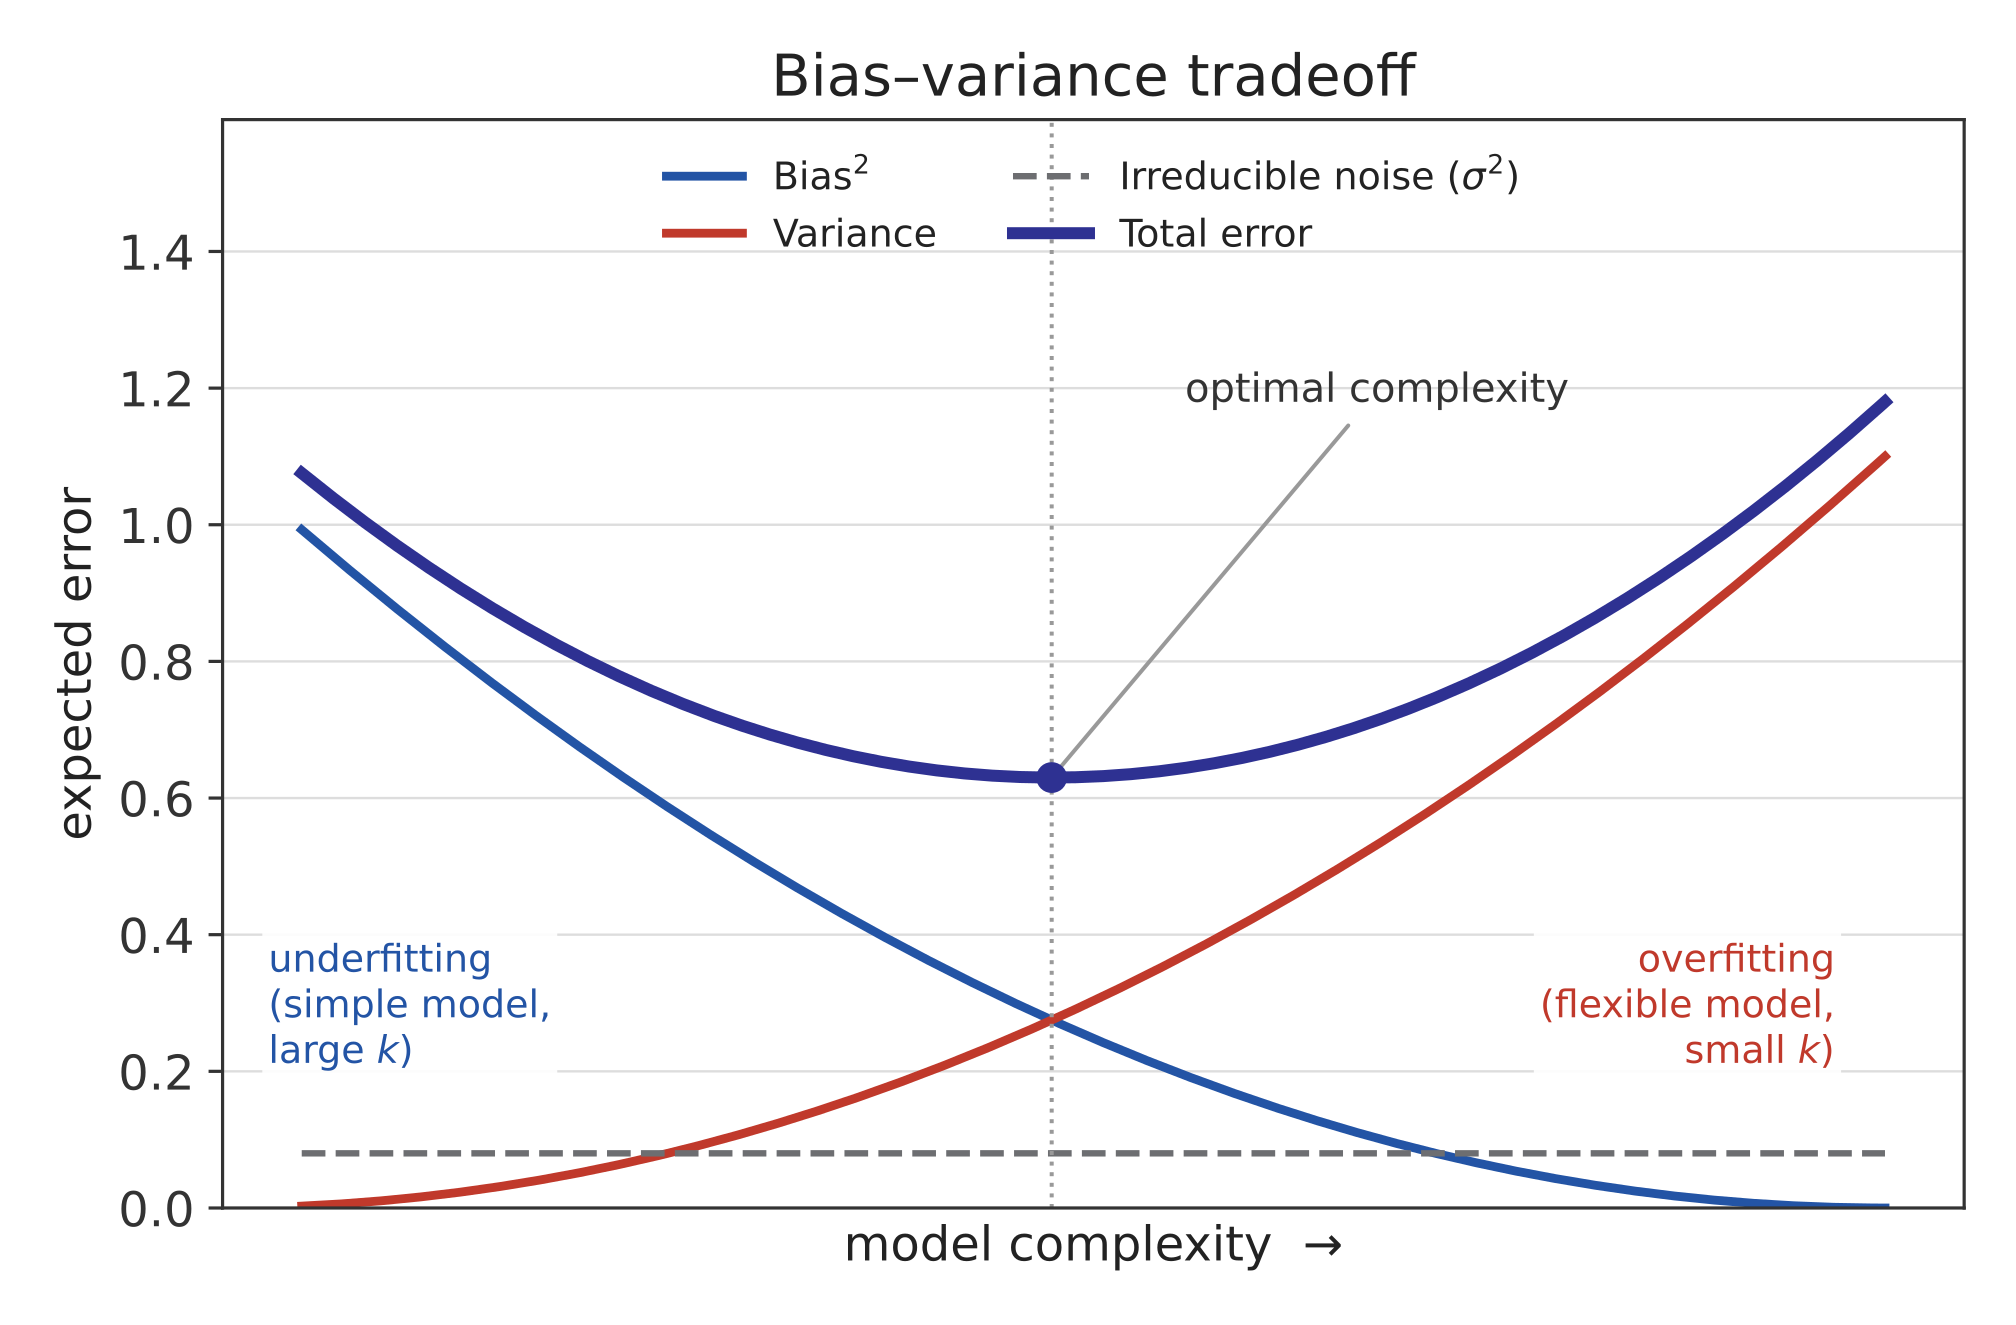
\includegraphics[width=\linewidth]{ch04_bias_variance.png}
    \end{column}
    \begin{column}{0.43\textwidth}
      \begin{itemize}\small
        \item \textbf{너무 단순}($k$ 큰 kNN, 얕은 트리, 규제가 강한
          선형모델) $\to$ Bias↑, Variance↓ = \textbf{과소적합}
        \item \textbf{너무 유연}($k{=}1$ kNN, 아주 깊은 트리,
          대형 신경망) $\to$ Variance↑, Bias↓ = \textbf{과적합}
        \item 최적 모델 복잡도 = 둘의 합(전체 오차)이 \textbf{최소}
          되는 지점
        \item 이 프레임은 Ch.\,6(정규화), Ch.\,7(트리 가지치기),
          Ch.\,9(신경망 정규화)에서 ``과적합을 어떻게 막나''를
          다룰 때마다 다시 등장
      \end{itemize}
    \end{column}
  \end{columns}
\end{frame}

\begin{frame}{``분산이 크다''의 구체적 그림}
  진짜 경계가 대각선으로 갈라진 두 덩어리, 경계 근처에 \textbf{한
  점만} 잘못 찍혀 있다고 하자:
  \vskip0.8em
  \begin{columns}[T]
    \begin{column}{0.48\textwidth}
      \kb{$k=1$}
      \begin{itemize}\small
        \item 잘못 찍힌 점 바로 옆에서 ``그 점이 정답''
        \item \textbf{경계 전체가 한 점의 위치를 따라 출렁}
      \end{itemize}
    \end{column}
    \begin{column}{0.48\textwidth}
      \kb{$k=5$}
      \begin{itemize}\small
        \item 잘못 찍힌 한 점을 4개 정상점이 \textbf{투표로 이김}
        \item 그 한 점은 경계에 거의 영향 없음
      \end{itemize}
    \end{column}
  \end{columns}
  \vskip0.8em
  반대로 진짜 경계가 \textbf{복잡하게 꼬여} 있으면, $k=5$는
  ``이웃 5개 다수결''로 세부 곡선을 따라가지 못하고 매끄럽게
  그은다 --- 이쪽은 \kb{편향}의 문제.
  \vskip0.6em
  \begin{block}{정의의 kNN 번역}
    분산이 크다 = \textbf{훈련 데이터의 미세한 변화}(노이즈 한 점,
    표본 재추출)가 \textbf{예측의 미세한 변화}(경계의 출렁임)를
    낳는 정도. kNN에서는 이 인과가 \textbf{눈으로 직접 확인}
    가능 --- 신경망에서 ``분산''을 눈으로 보기 훨씬 어렵다.
  \end{block}
\end{frame}

\begin{frame}[fragile]{손으로 한 번: kNN 예측 직접 계산}
  학습 데이터 6개, 두 반(불합격 0 / 합격 1):
  \[(1,1)\to0,\ (2,1)\to0,\ (1,2)\to0,\ (8,8)\to1,\ (9,8)\to1,\ (8,9)\to1\]
  새 점 $(7,7)$을 $k=3$으로 분류 --- 유클리드 거리 계산:
  \small
  \begin{tabular}{@{}lll@{}}
    \toprule
    학습 데이터 & 라벨 & $(7,7)$까지 거리 \\
    \midrule
    (8,8) & 1 & $\sqrt{2}\approx1.414$ \\
    (9,8) & 1 & $\sqrt{5}\approx2.236$ \\
    (8,9) & 1 & $\sqrt{5}\approx2.236$ \\
    (2,1) & 0 & $\sqrt{61}\approx7.810$ \\
    (1,2) & 0 & $\sqrt{61}\approx7.810$ \\
    (1,1) & 0 & $\sqrt{72}\approx8.485$ \\
    \bottomrule
  \end{tabular}
  \vskip0.8em
  가장 가까운 3개 --- (8,8), (9,8), (8,9) --- 가 \textbf{모두
  라벨 1} $\Rightarrow$ 다수결로 $(7,7)$은 \kb{1(합격)}.
  \vskip0.4em
  \texttt{knn\_predict}가 정확히 이 정렬·다수결 과정을 자동화한 것.
  \textbf{회귀}로 보면: 같은 라벨을 $1,1,1,4,4,4$로 두면 가장 가까운
  3개 라벨의 평균 $(4+4+4)/3 = 4.0$ --- \textbf{같은 $k$개의
  이웃}을 쓰고, 집계 방식(다수결 vs 평균)만 다르다.
\end{frame}

\begin{frame}{결정경계: $k$를 키우면 어떻게 변하나}
  \begin{columns}[T]
    \begin{column}{0.55\textwidth}
      \centering
      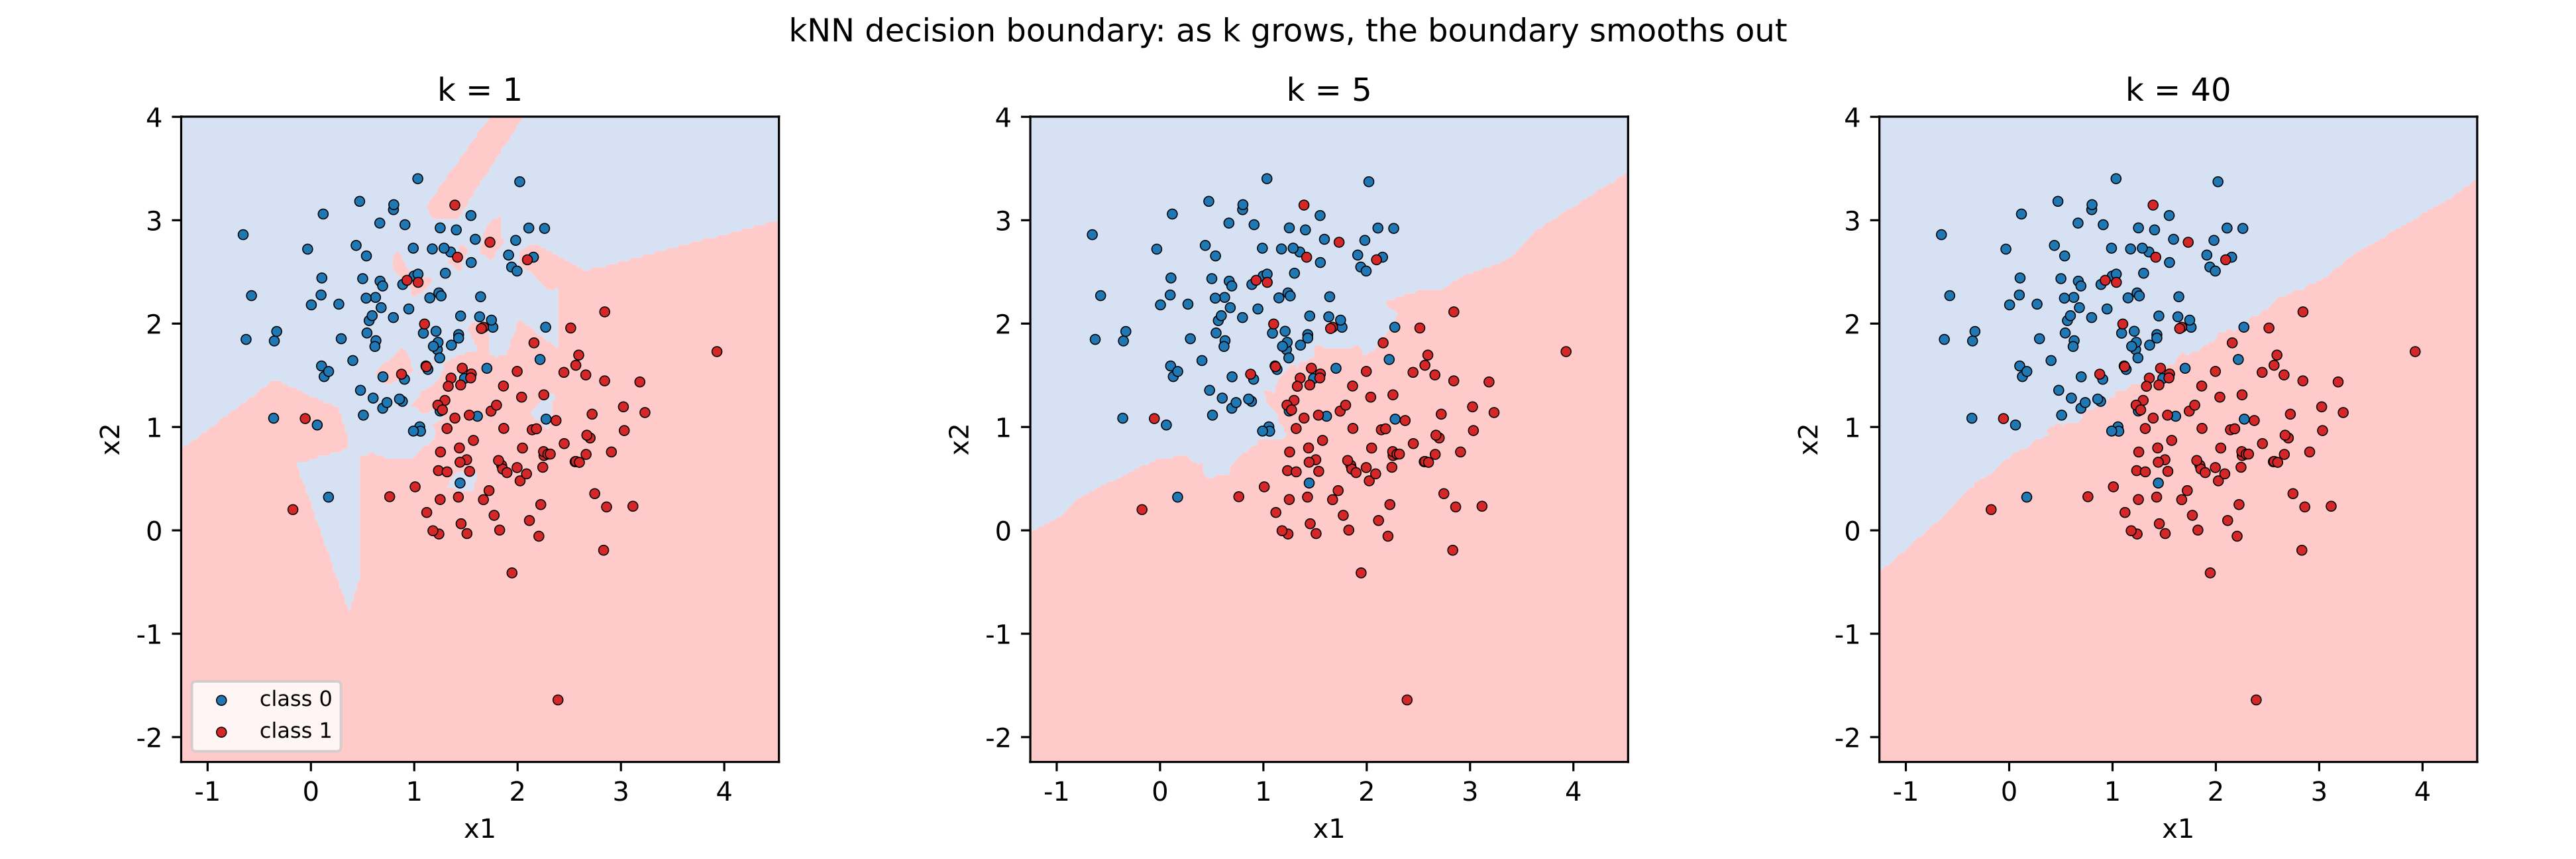
\includegraphics[width=\linewidth]{ch04_knn_decision_boundary.png}
    \end{column}
    \begin{column}{0.43\textwidth}
      \begin{itemize}\small
        \item 두 원형 blob(클래스 0: 왼쪽 위, 1: 오른쪽 아래) 200개
          점, $k=1,5,40$의 결정경계
        \item \kb{$k=1$}: 훈련점 주변에 \textbf{톱니바퀴}처럼
          복잡하게 접힘 --- 각 점의 ``영향권''(보로노이 셀) 경계가
          그대로 결정경계
        \item \kb{$k=5$}: 톱니가 눈에 띄게 \textbf{매끄러워짐}
          (한두 점의 노이즈는 5표에서 다수결을 못 뒤집음)
        \item \kb{$k=40$}(훈련점 140개 중 1/3): \textbf{거의
          직선} $\to$ 지역 패턴 무시, 과소적합의 공간적 모습
      \end{itemize}
    \end{column}
  \end{columns}
  \vskip0.6em
  매끄러움이 어느 시점부터는 \textbf{정보를 잃는 매끄러움}
  (진짜 패턴 지우기)이 되는지 = \textbf{검증 정확도}로 판단
  (4.2절에서 실제로 $k$ 튜닝).
\end{frame}

\begin{frame}{기하학적 성격: 보로노이 다이어그램}
  \begin{itemize}
    \item \kb{$k=1$ kNN의 결정경계 = \kb{보로노이 다이어그램}의 경계}
      (Voroni, 1908)과 정확히 일치
    \item \kb{보로노이 셀}: 특정 훈련점 $x_i$에 가장 가까운 모든
      지점들의 영역 $\{x : d(x, x_i) \le d(x, x_j)\ \forall j\}$
      --- 각 $x_i$를 중심으로 한 \textbf{볼록 다각형}, 이웃 셀 경계는
      두 점의 \textbf{수직등분선}
  \end{itemize}
  \vskip0.8em
  \begin{block}{두 가지 실용적 의미}
    \begin{enumerate}\small
      \item $k=1$ 경계는 \textbf{항시 각진(비선형) 다각형의 합} ---
        아무리 많은 점을 써도 \textbf{곡선을 그을 수 없다}(충분히
        작은 직선 조각으로만 근사)
      \item \textbf{두 훈련점이 아주 가까우면} 그 수직등분선이
        두 점 사이를 지나, 근처 경계가 두 점의 \textbf{상대적 위치
       에만} 달려 있다 = 분산 얘기의 기하학적 번역
    \end{enumerate}
  \end{block}
  $k>1$에서는 \kb{$k$-보로노이}가 경계를 정의 --- ``$k$-이웃의
  클래스 분포가 50:50으로 바뀌는 곳''. $k$가 커질수록 매끄러워진다는
  직감의 기하학적 근거.
\end{frame}

\begin{frame}{자주 하는 실수: 스케일이 다른 특징을 그대로 섞기}
  ``공부 시간''(1$\sim$9)과 ``가구 소득''(5000$\sim$6000만 원)으로
  합격을 예측 --- 학습점 $P_1=(9,\,5000)$(합격),
  $P_2=(1,\,5050)$(불합격), 새 점 $(8,\,6000)$:
  \[
  d(P_1, \text{new}) \approx 1000.0005, \qquad
  d(P_2, \text{new}) \approx 950.026
  \]
  \vskip0.4em
  \kq{소득 축이 거리를 독차지해 $P_2$가 오히려 더 가깝게} ---
  직관(공부시간 8 vs 9)과 정반대.
  \vskip0.6em
  0$\sim$1 정규화($P_1\to(1.0,0.0)$, $P_2\to(0.0,0.05)$,
  $\text{new}\to(0.875,1.0)$)하면:
  \[
  d(P_1, \text{new}) \approx 1.008, \qquad d(P_2, \text{new}) \approx 1.292
  \]
  정규화 후에는 $P_1$이 더 가까워 \textbf{뒤집힌다} --- 직관과
  일치. \texttt{StandardScaler}나 \texttt{MinMaxScaler}
  (scikit-learn, Pedregosa et al.\ 2012)를 쓰는 것은 선형회귀의
  학습률 선택만큼이나 \textbf{기본적인 체크리스트 항목}.
\end{frame}

\begin{frame}{정규화의 효과, 숫자로: 0.556 $\to$ 1.000}
  두 클래스가 \textbf{$x$축 하나}로만 분리되는 데이터:
  클래스 0은 $x\approx0.5$, 클래스 1은 $x\approx0.1$,
  $y$축은 두 클래스 모두 $5\pm3$의 잡음.
  $x$의 범위(약 0.6)가 $y$의 범위(약 9)에 비해 매우 작다.
  \vskip0.8em
  \small
  \begin{tabular}{@{}lc@{}}
    \toprule
    & 검증 정확도 ($k=3$) \\
    \midrule
    정규화 \textbf{없이} & 0.556 \\
    정규화 \textbf{후} & \textbf{1.000} \\
    \bottomrule
  \end{tabular}
  \vskip1em
  \begin{block}{해석}
    ``$y$ 잡음으로만 분류하던 모델''이 정규화 후 $x$가 분리 축으로
    정상 작동 $\to$ 정확도 \textbf{거의 두 배}. 정규화 없이
    성능이 40\%나 깎일 수 있는 \textbf{극단적 사례} ---
    센서·금융 데이터 등 실데이터에서 이런 스케일 차이는 흔하다.
  \end{block}
\end{frame}

\begin{frame}{베이스라인으로서의 kNN}
  \begin{itemize}
    \item \textbf{과거}: 1967년 Cover--Hart(이론적으로만 안전할 뿐 실용성
      낮다)로 잊혔다가, 1998년 \kb{MNIST}(LeCun et al.\ 1998) 시대
      kNN이 \textbf{약 97\%}(오류율 약 3\%)를 기록하며
      ``복잡한 모델 없이 경쟁력 있는 베이스라인''으로 재등장
    \item \textbf{현대}: 큰 데이터셋에서 예측 $O(m\cdot d)$라
      느리다는 단점이 명확해 CNN(Ch.\,10)·신경망(Ch.\,9)에 자리를
      내줬지만, \textbf{베이스라인}으로 여전히 쓰임
  \end{itemize}
  \vskip0.8em
  \begin{block}{정석}
    ``새 데이터셋을 받았다, 어떤 모델을 써볼까?''
    $\to$ \textbf{먼저 kNN으로 베이스라인을 잡아봐라}.
    \begin{itemize}\small
      \item kNN은 가정이 거의 없으므로 데이터의
        \textbf{``학습 가능성'' 하한}을 알려줌
      \item kNN으로조차 좋은 성능이 안 나오면 더 복잡한 모델도
        (거의) 확실히 어려움 = \textbf{조기 경보기}
      \item kNN으로 90\%를 나갔다면, 더 복잡한 모델은
        \textbf{그 90\%를 초과해야} 의미가 있음
    \end{itemize}
  \end{block}
\end{frame}

\begin{frame}{자주 묻는 질문 (4.1)}
  \small
  \begin{itemize}
    \item \textbf{Q. 왜 ``학습이 없다''고 하나요?}
      선형회귀는 데이터를 $w$ 몇 개로 \textbf{압축}해 저장,
      kNN은 \textbf{원본 전체}를 갖고 있어야 예측 가능 ---
      파라미터 최적화 과정 자체가 없음
    \item \textbf{Q. $k$는 항상 홀수?}
      이진 분류에선 동점(2:2) 방지를 위해 홀수가 관례적.
      클래스 $\geq 3$개면 홀수여도 동점이 날 수 있어
      \textbf{동점 처리 규칙}을 미리 정해두는 것이 안전
    \item \textbf{Q. kNN으로 회귀를 해도 되나요?}
      된다 --- ``가장 가까운 $k$개 $y$의 평균'' =
      \textbf{국소적 평균 smoother}, 비모수 회귀의 가장
      기본적인 형태(신경망이 ``복잡한 비모수 근사''라면
      kNN 회귀는 ``가장 단순한 비모수 근사'').
      단, 차원이 높아지면(4.2) 이웃 평균이 노이즈에
      완전히 지배됨
    \item \textbf{Q. 예측 확률 $P(y=1|x)$는?}
      가장 가까운 $k$개 중 \textbf{클래스 1의 비율}
      $\hat P(y=1|x) = \frac{\#\{\text{클래스 1 이웃}\}}{k}$
      --- 다수결 분류기의 확률적 버전(0.5 초과 시 1로 예측).
      $k$가 클수록 안정적, 실전에선 거리 가중
      ($w_i = 1/d^2$ 등)으로 고치기도
    \item \textbf{Q. 특징 100개 넘으면?}
      쓸 수는 있으나 \textbf{성능이 크게 떨어짐}(차원의 저주).
      실전 고차원 kNN = \textbf{특징 선택} 또는
      \textbf{차원 축소}(Ch.\,14 PCA)를 먼저 --- 표준적 절차.
      특징 10개 미만의 저차원 데이터라면 여전히 경쟁력
  \end{itemize}
\end{frame}

\begin{frame}{실습으로 연결하기 (4.1)}
  노트북 \texttt{chapter04\_1\_knn.ipynb}에서:
  \begin{enumerate}
    \item 두 blob 데이터에 kNN을 적용,
      \textbf{$k=1, 5, 40$의 결정경계를 나란히} 그림
    \item 같은 데이터에 $k$를 1$\to$40까지 쭉 늘리며
      \textbf{훈련 정확도 vs 검증 정확도} 그래프 ---
      ``과적합 $\to$ 정상 $\to$ 과소적합'' 궤적을 직접 관찰
    \item 1차원 $\sin$ 함수 + 잡음 데이터에서
      \textbf{편향·분산을 수치적으로 측정}
      (앞 표의 숫자가 여기서 나옴)
    \item 스케일이 다른 특징 데이터를
      \textbf{정규화 전/후}로 나누어 kNN 정확도 비교
      (0.556 vs 1.000 예시가 여기서 나옴)
  \end{enumerate}
\end{frame}

% ============================================================
\section{4.2 차원의 저주와 실습: 검증셋으로 k 튜닝하기}

\begin{frame}{차원의 저주: ``가까운 이웃''이 멀어진다}
  \kq{특징이 늘어날수록, ``가장 가까운 이웃''조차 점점 멀어진다.}
  \vskip0.8em
  \begin{itemize}
    \item kNN의 전제 = ``가까운 데이터는 \textbf{비슷한 답}을
      가질 것이다'' --- 특징이 수백 개가 되면 이 직관이 무너짐
    \item \textbf{원인은 부피}: $n$차원에서 한 변을 0.5로만 줄여도
      부피가 $0.5^n$으로 --- $n=100$이면 $10^{-30}$,
      \textbf{기하급수적으로 증발}
    \item 반대로 ``전체 부피의 일부''를 잡으려면 한 변을 거의 1에
      가깝게 늘려야 함
  \end{itemize}
  \vskip0.8em
  $n$차원 단위 정육면체 $[0,1]^n$에 점이 균등 분포,
  전체의 비율 $p$를 포함하려면 한 변 $\ell$:
  \[
  \ell^n = p \quad\Longrightarrow\quad \ell = p^{1/n}
  \]
  \kq{$p=0.01$(전체의 1\%)일 때의 $\ell$:}
  \small
  \begin{tabular}{@{}ccc@{}}
    \toprule
     $n$ & $\ell = p^{1/n}$ & \\
    \midrule
    1  & 0.01 & \\
    10 & 0.63 & \\
    100 & 0.955 & \textbf{각 변 길이의 95.5\%나} 차지해야 겨우 1\% \\
    \bottomrule
  \end{tabular}
\end{frame}

\begin{frame}{동거리 현상: 순서가 무너진다}
  \begin{itemize}
    \item \kb{이웃들이 ``모두 비슷한 거리''에 놓이는 현상}
      (거리 집중, distance concentration)
    \item kNN은 이웃을 \textbf{순서대로}(1번째, 2번째, …) 고르는
      알고리즘 $\Rightarrow$ 순서가 의미를 잃으면 \textbf{치명적}
  \end{itemize}
  \vskip0.6em
  단위 정육면체에 200개 점 균등 분포, 20개 임의 질의점에서
  ``1번째''와 ``11번째'' 이웃까지의 평균 거리:
  \small
  \begin{tabular}{@{}cccc@{}}
    \toprule
     $n$ & 1번째 이웃 & 11번째 이웃 & 비율(11/1) \\
    \midrule
    2  & 0.033 & 0.142 & \textbf{4.33} \\
    5  & 0.253 & 0.514 & 2.04 \\
    10 & 0.617 & 0.894 & 1.45 \\
    20 & 1.151 & 1.429 & 1.24 \\
    50 & 2.246 & 2.509 & \textbf{1.12} \\
    \bottomrule
  \end{tabular}
  \vskip0.8em
  2차원에서 4.3배였던 차이가 50차원이면 1.12배 $\to$
  \textbf{거리라는 정보만으로 이웃을 차별화할 수 없게} 된다.
  kNN이 ``가장 가까운 $k$개''를 고른다고 믿는 근거가
  허공을 가리키는 셈.
\end{frame}

\begin{frame}{동거리의 수학적 근거: $k^{1/n}$ 스케일}
  핵심: \textbf{거리가 차원에 $1/n$승 지수로} 붙는다.
  $n$차원에서 ``부피의 $f$ 비율을 덮는 구''의 반지름은
  $f^{1/n}$ 스케일 $\Rightarrow$ $k$번째 이웃까지의 거리
  $\ell_k \propto (k/m)^{1/n}$.
  \vskip0.6em
  $m$ 고정, $k$만 바꾸면 \textbf{$k$번째/1번째 이웃 거리 비율}은
  \textbf{$k^{1/n}$} ($m$과 상수계수는 약분으로 사라짐).
  시뮬레이션의 ``11번째/1번째'' 열($k=11$)과 비교:
  \small
  \begin{tabular}{@{}ccc@{}}
    \toprule
     $n$ & 이론 $11^{1/n}$ & 시뮬레이션 \\
    \midrule
    2  & 3.32 & 4.33 \\
    10 & 1.27 & 1.45 \\
    50 & 1.05 & 1.12 \\
    \bottomrule
  \end{tabular}
  \vskip0.8em
  이론값이 측정값보다 꾸준히 약간 작긴 하지만(가장자리 효과),
  \textbf{$n$이 커지며 1로 수렴하는 모양은 정확히 같음} ---
  $1/n$ 지수가 $n\to\infty$에서 0에 붙어 모든 순서의 이웃이
  1에 수렴하기 때문.
\end{frame}

\begin{frame}{실험: 노이즈 특징을 붙여가면?}
  2차원 \kb{moons}(반달 두 개) 데이터, $k=7$ 고정,
  \textbf{정보 하나도 담지 않는} 잡음 특징을 0$\to$5$\to$20$\to$50개
  붙여가며 검증 정확도 측정:
  \small
  \begin{tabular}{@{}lc@{}}
    \toprule
    잡음 특징 수 (총 차원) & 검증 정확도 ($k=7$) \\
    \midrule
    0 (2차원)  & \textbf{0.867} \\
    5 (7차원)  & 0.813 \\
    20 (22차원) & 0.680 \\
    50 (52차원) & \textbf{0.507} \\
    \bottomrule
  \end{tabular}
  \vskip1em
  \begin{block}{해석}
    52차원이면 \textbf{0.507} --- 동전 던지기(0.500)와 사실상
    무차이. 원래 들어 있던 \textbf{유용한 2차원 신호는 그대로}인데,
    \textbf{아무것도 알려주지 않는 축 50개}를 추가했을 뿐
    $\Rightarrow$ 순수하게 차원의 저주만으로 정확도가 \textbf{무너짐}.
    ``특징을 더 많이 모은 것''이 오히려 \textbf{해로운 축}을 추가한 셈.
  \end{block}
  \kq{차원의 저주는 ``차원의 \textbf{숫자}''가 아니라,
  거리에 \textbf{노이즈 축이} 얼마나 섞여 있는가}에 달려 있다.
\end{frame}

\begin{frame}{역사: 용어의 기원 (Bellman 1957)}
  ``\kb{차원의 저주}(curse of dimensionality)''라는 용어는
  리처드 벨만이 1957년경 \textbf{동적계획법} 관련 저작에서
  처음 썼다.
  \vskip0.8em
  \begin{itemize}
    \item 그가 말한 것은 \textbf{계산 비용} 문제:
      ``$n$이 늘어남에 따라 필요한 연산량이 기하급수적으로
      증가한다''
    \item 지금처럼 ``고차원에서 데이터가 \textbf{희소}해지고,
      \textbf{거리 기반 추론}이 무너진다''는 \textbf{데이터
      기하학} 문제로 확장된 것은 이후 ML·통계 문맥에서의 발전
  \end{itemize}
  \vskip0.8em
  \begin{block}{이력이 주는 교훈}
    ``왜 느려지는가''(계산 복잡도)에서 ``왜 정확도가 무너지는가''
    (데이터 희소성)로 의미가 넓혀진 이 사실은, 우리가 다루는 것이
    본질적으로 \textbf{기하학적/데이터적 문제}(인접한 점들이
    동거리에 놓임)라는 점을 상기시켜 준다 --- 계산 효율의 문제가
    아니라, \textbf{공간 자체가} $n$차원이 되면서 변하는 성질.
  \end{block}
\end{frame}

\begin{frame}{자주 묻는 질문 (4.2-a)}
  \small
  \begin{itemize}
    \item \textbf{Q. 차원의 저주는 kNN에만 해당하나요?}
      아니다 --- \textbf{거리/유사도를 직접 재는 모든 방법}
      (k-means, 커널 SVM, PCA 이전 원본 공간의 유사도 등)이
      정도만 다를 뿐 같은 문제. 반면 \textbf{트리 기반}은
      한 번에 특징 하나씩만 보고 나누므로 상대적으로 덜 취약.
      ``이 모델이 거리를 직접 쓰는가?''가 취약도를 가늠
    \item \textbf{Q. 차원이 많으면 항상 특징을 줄여야 하나?}
      \textbf{꼭 그렇지는 않다} --- 유용한 정보가 소수 축에
      몰려 있으면 \textbf{특징 선택/차원 축소}(PCA)가 도움.
      반대로 각각이 \textbf{독립적으로 유의미한 신호}를 담고
      있으면(Ch.\,3 나이브베이즈가 바로 이런 설계) 무작정
      줄이는 것이 오히려 정보 손실
  \end{itemize}
\end{frame}

\begin{frame}{자주 묻는 질문 (4.2-b): 속도/메모리는 별개의 문제}
  \small
  \begin{itemize}
    \item \textbf{Q. 고차원에서는 ``속도''도 문제되지 않나요?}
      된다 --- 그리고 이는 정확도 문제(동거리)와
      \textbf{서로 다른} 문제. 순진한 구현은 예측 1번에
      $O(m \cdot n)$ 연산: $m=10^6, n=100$이면 약 $10^8$ 회
      곱셈/덧셈 --- numpy로 0.1초 이내, 순수 Python 루프로는
      수 초
    \item 더 큰 문제는 \textbf{메모리}: $10^6$개 점의 좌표를
      double(8바이트)로 저장 = $8\times10^8$ 바이트
      $\approx$ \textbf{800MB} + 예측 시점의 중간 배열
    \item 실전에서는 \kb{k-d 트리}(Friedman, 1970) 같은 탐색
      가속 자료구조를 쓰지만, 대략 $n > 20$ 이상에서는 탐색
      효율이 급격히 떨어져 \textbf{선형 탐색과 비슷}해짐
  \end{itemize}
  \vskip0.6em
  \begin{block}{정리}
    ``고차원에서는 kNN이 느리다'' = \textbf{정확도} 문제와
    \textbf{속도/메모리} 문제가 \textbf{독립적으로} 모두 성립하는
    두 가지의 합.
  \end{block}
\end{frame}

\begin{frame}{실습: 검증셋으로 k 튜닝}
  4.1절에서 ``적절한 $k$는 검증 데이터로 정한다''고 했다
  --- 직접 해보자.
  \begin{enumerate}\small
    \item 데이터를 \textbf{훈련/검증}으로 분리
    \item 여러 $k$ 각각에 대해 \textbf{검증셋 정확도} 계산
    \item 가장 높은 지점을 고른다
  \end{enumerate}
  \vskip0.6em
  \texttt{make\_moons}(scikit-learn) 500개 점, 30\% 검증 /
  70\% 훈련, $k \in \{1,3,5,7,10,15,20,30,50\}$:
  \small
  \begin{tabular}{@{}ccc@{}}
    \toprule
     $k$ & 훈련 정확도 & 검증 정확도 \\
    \midrule
    1  & \textbf{1.000} & 0.900 \\
    5  & 0.940 & 0.920 \\
    7  & 0.931 & \textbf{0.960} \\
    15 & 0.934 & 0.947 \\
    30 & 0.929 & 0.947 \\
    50 & 0.920 & 0.933 \\
    \bottomrule
  \end{tabular}
  \vskip0.8em
  $k=1$: 훈련 100\%에 가깝지만(과적합) 검증은 오히려 떨어짐 ---
  편향-분산 트레이드오프가 숫자로 드러나는 지점.
  검증 정확도는 $k$가 작을 때(분산)와 클 때(편향)
  \textbf{양쪽 끝에서 모두 낮아지는 ``U'' 모양}.
  이 표에선 $k=7$(0.960)이 최고.
\end{frame}

\begin{frame}[fragile]{tune\_k 코드}
\begin{lstlisting}
def train_val_split(X, y, val_ratio=0.3, seed=0):
    import random
    idx = list(range(len(X)))
    random.Random(seed).shuffle(idx)
    n_val = int(len(X) * val_ratio)
    val_idx, train_idx = idx[:n_val], idx[n_val:]
    return ([X[i] for i in train_idx], [y[i] for i in train_idx],
            [X[i] for i in val_idx], [y[i] for i in val_idx])

def tune_k(X, y, k_candidates):
    X_train, y_train, X_val, y_val = train_val_split(X, y)
    best_k, best_acc = None, -1.0
    for k in k_candidates:
        correct = sum(knn_predict(X_train, y_train, xv, k) == yt
                      for xv, yt in zip(X_val, y_val))
        acc = correct / len(X_val)
        if acc > best_acc:
            best_k, best_acc = k, acc
    return best_k
\end{lstlisting}
  핵심: 정확도를 \texttt{X\_val, y\_val}(학습에 안 쓴 데이터)
  로만 측정 --- 훈련 데이터 자체의 정확도로 고르면 4.1절의
  함정에 빠진다(다음 프레임).
\end{frame}

\begin{frame}[fragile]{자주 하는 실수: 훈련 정확도로 k 고르기}
  \begin{alertblock}{실수: 훈련 데이터 자체의 정확도로 $k$를 고르면}
\begin{lstlisting}
# ❌ 실수: 훈련 데이터 자체의 정확도로 k를 고르는 함수
def tune_k_wrong(X, y, k_candidates):
    X_train, y_train, X_val, y_val = train_val_split(X, y)
    best_k, best_acc = None, -1.0
    for k in k_candidates:
        acc = sum(knn_predict(X_train, y_train, xt, k) == yt
                  for xt, yt in zip(X_train, y_train)) / len(X_train)
        if acc > best_acc:
            best_k, best_acc = k, acc
    return best_k   # -> 항상 1 이 반환된다
\end{lstlisting}
  \end{alertblock}
  \begin{itemize}
    \item 이 함수를 돌리면 $k=1$이 ``최고''로 나온다
    \item $k=1$일 때 각 훈련점에 대해 ``가장 가까운 1개''는
      \textbf{자기 자신} $\Rightarrow$ 훈련 정확도 \textbf{정확히
      1.000}, 그 어떤 $k$도 이를 넘을 수 없음
  \end{itemize}
  \vskip0.6em
  \kq{훈련 정확도를 최대화하는 $k$는 구조적으로 언제나 $k=1$}
  --- 데이터를 통째로 외운 것과 다름없다.
\end{frame}

\begin{frame}{확인 문제: $\ell$를 직접 계산}
  앞 표에선 $n=1,10,100$만 계산했다 ---
  \textbf{$n=20$일 때 $\ell = 0.01^{1/20}$은?}
  \vskip0.6em
  \begin{itemize}
    \item 계산기 전에 추정해보자: $n=10$일 때 0.63,
      $n=100$일 때 0.955였으니 $n=20$은 그 사이 어디쯤
    \item \textbf{힌트}: $\ell$가 $n$에 대해 \textbf{선형}으로
      늘어나는 게 아니라, $n$이 작을 때 \textbf{훨씬 빠르게}
      커진 뒤 1에 가까워지며 증가폭이 줄어듦에 주의
    \item 직접 \texttt{0.01 ** (1/20)}를 계산해 예상과 비교
      (참고값: $\approx 0.794$)
  \end{itemize}
  \vskip0.8em
  \begin{block}{이 숫자의 뜻}
    \textbf{특징이 20개만 되어도} ``근처 1\%''를 찾으려면 각 축의
    \textbf{대부분}(약 79\%의 비율)을 뒤져야 한다 ---
    겨우 20차원에서도 ``가까운 이웃''이라는 말이
    \textbf{이미 상당히 무뎌지기} 시작한다.
  \end{block}
\end{frame}

\begin{frame}{자주 하는 실수: 검증셋 없이 훈련 정확도로 k 고르기}
  \texttt{tune\_k}가 데이터를 훈련/검증으로 \textbf{굳이 나누는}
  이유를 실수 사례로 확인:
  \vskip0.8em
  \begin{itemize}
    \item 검증셋 없이 \textbf{훈련 데이터 자체}의 정확도로
      $k$를 고르면: $k=1$일 때 ``가장 가까운 1개''가 항상
      자기 자신 $\Rightarrow$ 훈련 정확도 \textbf{정확히 100\%}
      (데이터 통째로 외운 것과 다름없음)
    \item 이 기준으로 고르면 항상 $k=1$이 ``최고''로 보이지만,
      \textbf{정작 새로운 데이터}에서는 노이즈 하나에도
      흔들리는 \textbf{가장 불안정한} 선택
    \item \texttt{tune\_k}가 \texttt{X\_val, y\_val}(학습에 안
      쓴 데이터)로 정확도를 재는 이유가 정확히 이것을 막기
      위함
  \end{itemize}
  \vskip0.6em
  {\footnotesize Ch.\,6에서 이 원칙(모델을 고르는 데 쓰는 데이터
  와 최종 성능을 평가하는 데이터를 분리)을 train/val/test
  3분할로 더 엄밀하게 다룬다.}
\end{frame}

\begin{frame}{유명한 사례: MNIST의 첫 베이스라인}
  1998년 얀 르쿤(LeCun)이 손글씨 숫자 데이터셋 \kb{MNIST}를
  발표하면서, 비교 기준이 될 여러 알고리즘의 성능을 함께 보고했다.
  \vskip0.8em
  \begin{itemize}
    \item 그중 가장 단순한 축이 바로 \kb{kNN} ---
      별도 학습 과정도, 파라미터 튜닝도 거의 없이
      ``가장 비슷하게 생긴 숫자 이미지 몇 개를 찾아
      다수결로 정한다''는 방식만으로 \textbf{약 97\%}
      (오류율 약 3\%) 기록
    \item 이 챕터의 CNN(Ch.\,10)이 등장하기 전까지,
      ``복잡한 이론 없이 거리만 재는'' 이 단순한 방법이
      꽤 경쟁력 있는 \textbf{베이스라인}으로 쓰였음
  \end{itemize}
  \vskip0.8em
  \begin{block}{실용적 교훈}
    새 프로젝트를 시작할 때 \textbf{항상 복잡한 모델부터}
    시도할 필요는 없다 --- 가장 단순한 방법(kNN, 심지어
    평균/다수결)으로 \textbf{먼저 베이스라인}을 잡아두면,
    이후 더 복잡한 모델이 \textbf{정말로 그만한 값어치}를 하는지
    비교할 기준이 생긴다.
  \end{block}
\end{frame}

\begin{frame}{차원이 많으면 항상 특징을 줄여야 하나?}
  \textbf{꼭 그렇지는 않다} --- 답은 ``축들이 무엇을 담고 있는가''에
  달려 있다:
  \vskip0.8em
  \begin{columns}[T]
    \begin{column}{0.48\textwidth}
      \kb{유용한 신호가 소수 축에 몰려 있으면}
      \begin{itemize}\small
        \item 나머지 축이 노이즈에 가깝다면
        \item \textbf{특징 선택} 또는 \textbf{차원 축소}
          (Ch.\,14 PCA)로 의미 있는 축만 남기는 것이 도움
        \item = 앞 실험(50개 junk 축)의 정반대 상황
      \end{itemize}
    \end{column}
    \begin{column}{0.48\textwidth}
      \kb{각 축이 독립적으로 유의미한 신호를 담으면}
      \begin{itemize}\small
        \item 축이 많아도 무작정 줄이면 \textbf{정보 손실}
        \item Ch.\,3 \kb{나이브베이즈}가 바로 이런 상황을
          다루는 설계 --- ``특징 독립'' 가정으로 차원의 저주를
          \textbf{피해}내는 모델
      \end{itemize}
    \end{column}
  \end{columns}
  \vskip0.8em
  \kq{차원의 저주는 ``차원의 숫자''가 아니라,
  거리에 \textbf{노이즈 축}이 얼마나 섞여 있는가.}
\end{frame}

\begin{frame}{차원의 저주를 피하는 실전 해법 3가지}
  \begin{enumerate}
    \item \kb{특징 선택 / 차원 축소} ---
      PCA(Ch.\,14)나 도메인 지식을 이용해 \textbf{실제로 신호를
      담고 있는 축만} 남긴다
    \item \kb{모델 교체} --- 거리를 직접 재지 않는
      \textbf{트리 기반}(Ch.\,7) 또는 \textbf{선형 모델}로 넘어간다
      (트리는 한 번에 특징 하나씩만 보기 때문)
    \item \kb{거리의 ``유효 차원''을 낮추는 전처리} ---
      \textbf{정규화}(4.1절)를 적절히 하면 스케일이 큰 축이
      거리를 독차지하는 현상이 줄고, 실질적으로 유의미한
      차원의 수가 줄어드는 효과
  \end{enumerate}
  \vskip0.8em
  \begin{block}{어떤 해법이 맞는가}
    데이터에 따라 다르므로, Ch.\,6의 \textbf{교차검증}으로 각
    선택의 검증 정확도를 \textbf{직접 비교}해보는 것이
    가장 안전하다.
  \end{block}
\end{frame}

\begin{frame}{실습으로 연결하기 (4.2)}
  노트북 \texttt{chapter04\_2\_curse\_dim.ipynb}에서:
  \begin{enumerate}
    \item \textbf{동거리 시뮬레이션}(앞 표): 200개 점 균등 분포,
      20개 임의 질의점에서 1번째/11번째 이웃의 평균 거리를
      $n=2,5,10,20,50$로 실측
    \item \textbf{노이즈 특징 실험}(앞 표): moons 데이터에
      junk 축을 0$\to$50개 붙여가며 $k=7$ 검증 정확도
      0.867 $\to$ 0.507 추적
    \item \textbf{$k$ 튜닝 실습}: \texttt{tune\_k}로
      $k \in \{1,3,5,7,10,15,20,30,50\}$의 검증 정확도를 계산,
      최적 $k=7$(0.960) 확인 + \texttt{tune\_k\_wrong}이
      항상 $k=1$을 반환하는 함정 재현
  \end{enumerate}
\end{frame}

% ============================================================
\section{4.3 k-means 클러스터링}

\begin{frame}{비지도 클러스터링: 라벨 없이 거리만으로}
  \begin{columns}[T]
    \begin{column}{0.48\textwidth}
      \kb{kNN}(지도, 게으름)
      \begin{itemize}\small
        \item \textbf{라벨 있는} 학습점과 새 점의 거리만
          예측 시점에 재음
        \item ``새 점의 클래스 = 가까운 점의 다수결''
      \end{itemize}
    \end{column}
    \begin{column}{0.48\textwidth}
      \kb{k-means}(비지도)
      \begin{itemize}\small
        \item \textbf{라벨이 전혀 없는} 점들끼리
        \item ``서로 가까운 점은 한 덩어리''라는 거리 정보
          \textbf{만으로} 데이터의 구조를 쪼갬
        \item $k$개의 그룹, 각 그룹은 \kb{중심점}(centroid)으로
          대표
      \end{itemize}
    \end{column}
  \end{columns}
  \vskip0.8em
  \begin{block}{이 장의 축}
    라벨이 없다는 점에서 4.4절 \kb{GMM/EM}(k-means의 확률적
    일반화)과 직접 이어지지만, 핵심 동작(가장 가까운 대상을
    찾는다)은 이번 장의 주제 그대로.
  \end{block}
\end{frame}

\begin{frame}{k-means 알고리즘: 할당 $\to$ 갱신 반복}
  \begin{enumerate}
    \item $k$개의 중심점을 \textbf{무작위로 초기화}
    \item \kb{할당 단계}: 각 점을 \textbf{가장 가까운 중심점}의
      그룹으로 배정
    \item \kb{갱신 단계}: 각 그룹의 새 중심점 =
      그 그룹 점들의 \textbf{평균}
    \item 2$\sim$3을 \textbf{할당이 더 이상 바뀌지 않을
      때까지} 반복
  \end{enumerate}
  \vskip0.6em
  {\footnotesize 이 반복 절차의 기원 --- 1957년과 1967년의 두 번의
  독립적 발견 --- 이야기는 뒤의 ``유명한 사례''에서 다룬다.}
\end{frame}

\begin{frame}[fragile]{kmeans 코드}
\begin{lstlisting}
def kmeans(X, k, max_iters=100):
    import random
    centroids = random.sample(X, k)
    for _ in range(max_iters):
        clusters = [[] for _ in range(k)]
        for x in X:
            distances = [sum((x[j]-c[j])**2 for j in range(len(x)))
                         for c in centroids]
            closest = distances.index(min(distances))
            clusters[closest].append(x)
        new_centroids = [
            [sum(pt[j] for pt in cluster) / len(cluster)
             for j in range(len(X[0]))] if cluster else centroids[i]
            for i, cluster in enumerate(clusters)]
        if new_centroids == centroids:
            break
        centroids = new_centroids
    return centroids, clusters
\end{lstlisting}
  {\footnotesize \texttt{if cluster else centroids[i]}: 빈
  클러스터의 ``평균''은 정의되지 않으므로, 그 중심점을 그대로
  유지하는 것이 관례적 처리.}
\end{frame}

\begin{frame}{이 알고리즘이 뭘 최소화하는가: SSE}
  반복 과정 뒤에 숨은 목표 함수:
  \kb{클러스터 내 분산}(within-cluster sum of squares,
  \kb{SSE}):
  \[
  J = \sum_{i=1}^{k} \sum_{x \in C_i} \left\| x - \mu_i \right\|_2^2
  \]
  \begin{itemize}
    \item $C_i$ = $i$번 클러스터의 점 집합, $\mu_i$ = 그 중심점
    \item 해석: ``각 점이 \textbf{자기 그룹의 대표}까지
      \textbf{제곱해서} 얼마나 떨어져 있는가''의 합
    \item k-means = 이 $J$를 작게 만드는 \textbf{중심점과 분할}을
      찾는 알고리즘
  \end{itemize}
  \vskip0.6em
  \kq{``할당$\to$갱신''이라는 단순 반복이 실제로 $J$를 줄여가는
  \textbf{최적화 알고리즘}인가?} --- 각 단계의 간단한 수학으로
  보여준다.
\end{frame}

\begin{frame}{할당 단계가 $J$를 줄이는 이유}
  \begin{itemize}
    \item $J$는 각 점의 기여 $\|x - \mu_{\text{own}}\|^2$의 합
    \item 어떤 점이 자기 중심점에서 \textbf{다른} 중심점보다
      가까워졌다면, 그 점만 그 그룹으로 옮기면
      \textbf{해당 기여가 작아짐}
    \item $\Rightarrow$ 전체 합 $J$는 \textbf{줄거나 그대로}
  \end{itemize}
  \vskip0.8em
  \begin{block}{핵심}
    ``모든 점을 \textbf{가장 가까운} 중심점에게 배정한다''는
    규칙은, 정확히 \textbf{이 기여를 각 점마다 최소화}하는
    동작이다.
  \end{block}
\end{frame}

\begin{frame}{갱신 단계가 $J$를 줄이는 이유}
  한 클러스터의 점 $\{x_1, \dots, x_m\}$이 고정되어 있을 때,
  중심점 $c$에 대한
  \[
  f(c) = \sum_j \|x_j - c\|^2
  \]
  를 미분:
  \[
  \nabla_c f(c) = -2\sum_j (x_j - c) \quad =\; 0
  \iff c = \text{점들의 평균}
  \]
  \begin{itemize}
    \item 그래디언트가 \textbf{평균}일 때 정확히 0
    \item $f$는 $c$에 대해 \textbf{볼록한 이차함수}
      $\Rightarrow$ 이 안장점이 곧 \textbf{전역 최소점}
  \end{itemize}
  \vskip0.8em
  \begin{block}{결론}
    ``새 중심점 = \textbf{그룹의 평균}''은 해당 클러스터의 기여를
    최소화하는 \textbf{수학적으로 유일한 선택}.
  \end{block}
\end{frame}

\begin{frame}{수렴 보장 --- 그리고 그 한계}
  \begin{itemize}
    \item 두 단계가 \textbf{각각} $J$를 줄이므로, $J$는
      매 반복마다 \textbf{절대 늘어나지 않음}(단조감소)
    \item $J \geq 0$이고 점의 위치가 유한하므로
      $\Rightarrow$ 언젠가 \textbf{변화가 멈출 수밖에} 없다
      = \textbf{수렴 보장}의 전부
  \end{itemize}
  \vskip0.8em
  \begin{alertblock}{한계}
    이 보장은 $J$가 \textbf{어디까지} 줄어드는지에 대해
    \textbf{아무것도 말해주지 않는다}. 다른 초기화에서 출발하면
    다른 \textbf{``국소적 골짜기''}에 멈출 수 있다
    (\textbf{볼록하지 않은} 최적화 --- 4.1절 경사하강법과 같은
    구조). 그 결과가 곧 뒤의 ``자주 하는 실수''.
  \end{alertblock}
\end{frame}

\begin{frame}[fragile]{실습: 클러스터링 결과 시각화}
  2차원 데이터라면 할당 결과를 \textbf{눈으로} 바로 확인할 수
  있다 --- 알고리즘이 ``올바른'' 그룹을 찾았는지 감으로 검증하는
  가장 빠른 방법.
\begin{lstlisting}
import matplotlib.pyplot as plt

def plot_clusters(clusters, centroids):
    colors = ["tab:blue", "tab:orange", "tab:green", "tab:red"]
    for i, cluster in enumerate(clusters):
        xs = [pt[0] for pt in cluster]
        ys = [pt[1] for pt in cluster]
        plt.scatter(xs, ys, c=colors[i % len(colors)],
                    label=f"cluster {i}")
    plt.scatter([c[0] for c in centroids], [c[1] for c in centroids],
                c="black", marker="x", s=100, label="centroid")
    plt.legend()
    plt.savefig("kmeans_result.png")
\end{lstlisting}
  \vskip0.4em
  같은 데이터에 \texttt{k=2}, \texttt{k=3}, \texttt{k=4}를 돌려
  나란히 비교하면, ``몇 개의 덩어리로 나누는 게 자연스러운가''
  에 대한 감을 \textbf{숫자(SSE)보다 훨씬 빠르게} 얻을 수 있다.
\end{frame}

\begin{frame}{수렴 과정 시각화}
  \begin{columns}[T]
    \begin{column}{0.55\textwidth}
      \centering
      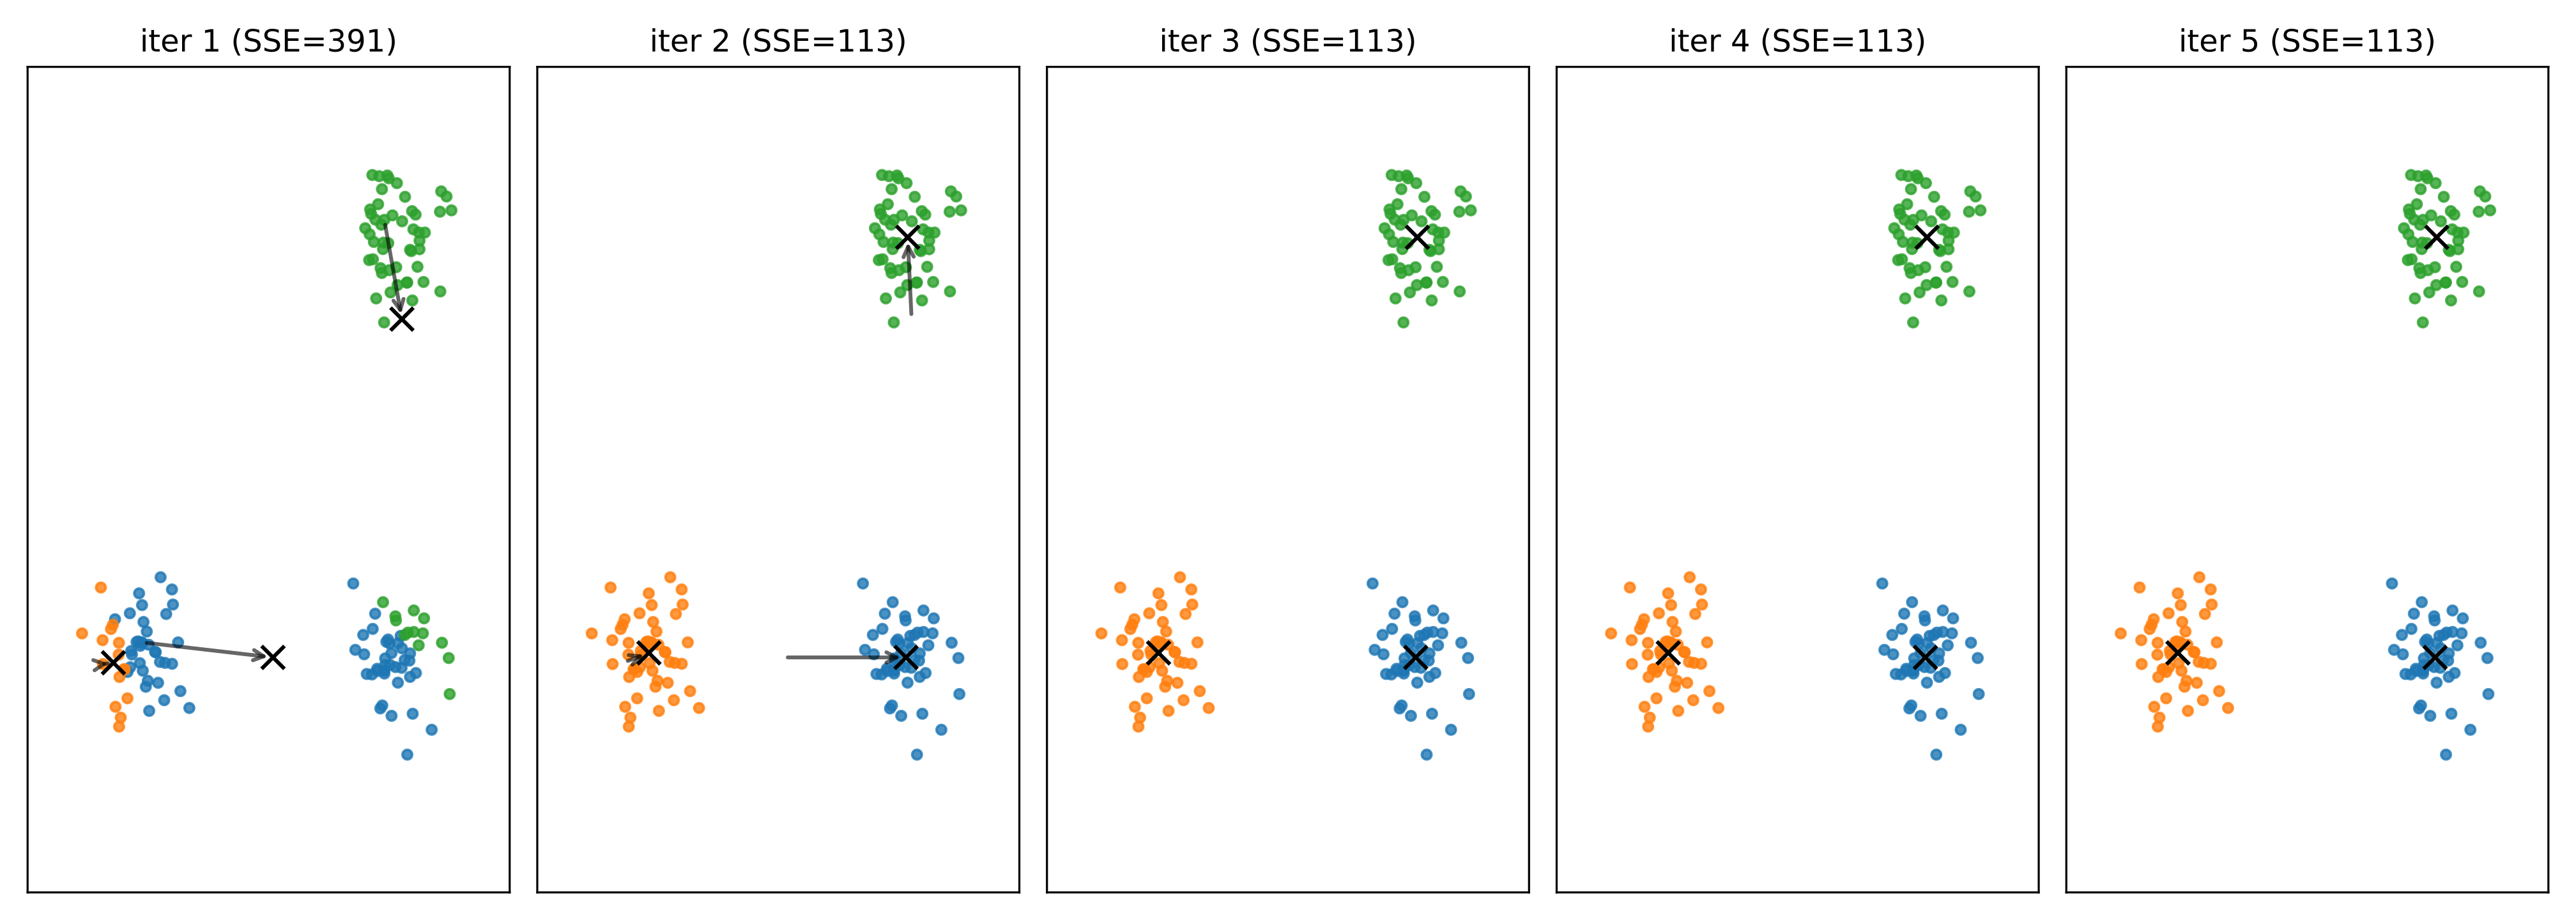
\includegraphics[width=\linewidth]{ch04_kmeans_convergence.png}
    \end{column}
    \begin{column}{0.43\textwidth}
      \begin{itemize}\small
        \item 150점 2차원 장난감 데이터(3개 원형 덩어리, 각 50점)
        \item 점의 색 = 할당된 클러스터, 검은 X = 그 회차의
          \textbf{중심점}, 화살표 = 이전$\to$이후 \textbf{중심점
          이동}
        \item 반복이 진행될수록 \textbf{화살표가 짧아지고}
          마지막 회차에는 \textbf{사라짐}
      \end{itemize}
      \vskip0.4em
      ``중심점이 \textbf{그룹의 평균}으로 재계산된다''는 문장을
      눈으로 확인할 수 있는 가장 빠른 방법.
    \end{column}
  \end{columns}
\end{frame}

\begin{frame}{k를 고르는 법: 엘보우(elbow) 방법}
  여러 $k$에 대해 \textbf{클러스터 내 분산}을 그려보고,
  \textbf{감소폭이 급격히 줄어드는 지점}(``팔꿈치'')을 고르는
  방법. 3-블롭 장난감 데이터(각 50점)에 $k=1\sim6$, 각
  무작위 초기화 10번 중 가장 작은 SSE:
  \small
  \begin{tabular}{@{}lcccccc@{}}
    \toprule
     $k$ & 1 & 2 & 3 & 4 & 5 & 6 \\
    \midrule
    SSE(최소) & 3753.3 & 1867.1 & \textbf{258.4} & 223.4 & 197.5 & 167.4 \\
    \bottomrule
  \end{tabular}
  \vskip1em
  \begin{itemize}
    \item $k=1\to2$: 거의 \textbf{반}으로 줄어듦(첫 분할)
    \item $k=2\to3$: \textbf{일곱 배 이상} 폭락(1867$\to$258) ---
      데이터에 실제로 \textbf{세 번째 덩어리}가 따로 존재
    \item $k=3\to4$: 겨우 35만 감소 --- 이미 ``진짜 구조''를 다
      건드렸고, 노이즈 수준에서 억지로 쪼갬
  \end{itemize}
\end{frame}

\begin{frame}{엘보우 곡선 읽기}
  \begin{columns}[T]
    \begin{column}{0.55\textwidth}
      \centering
      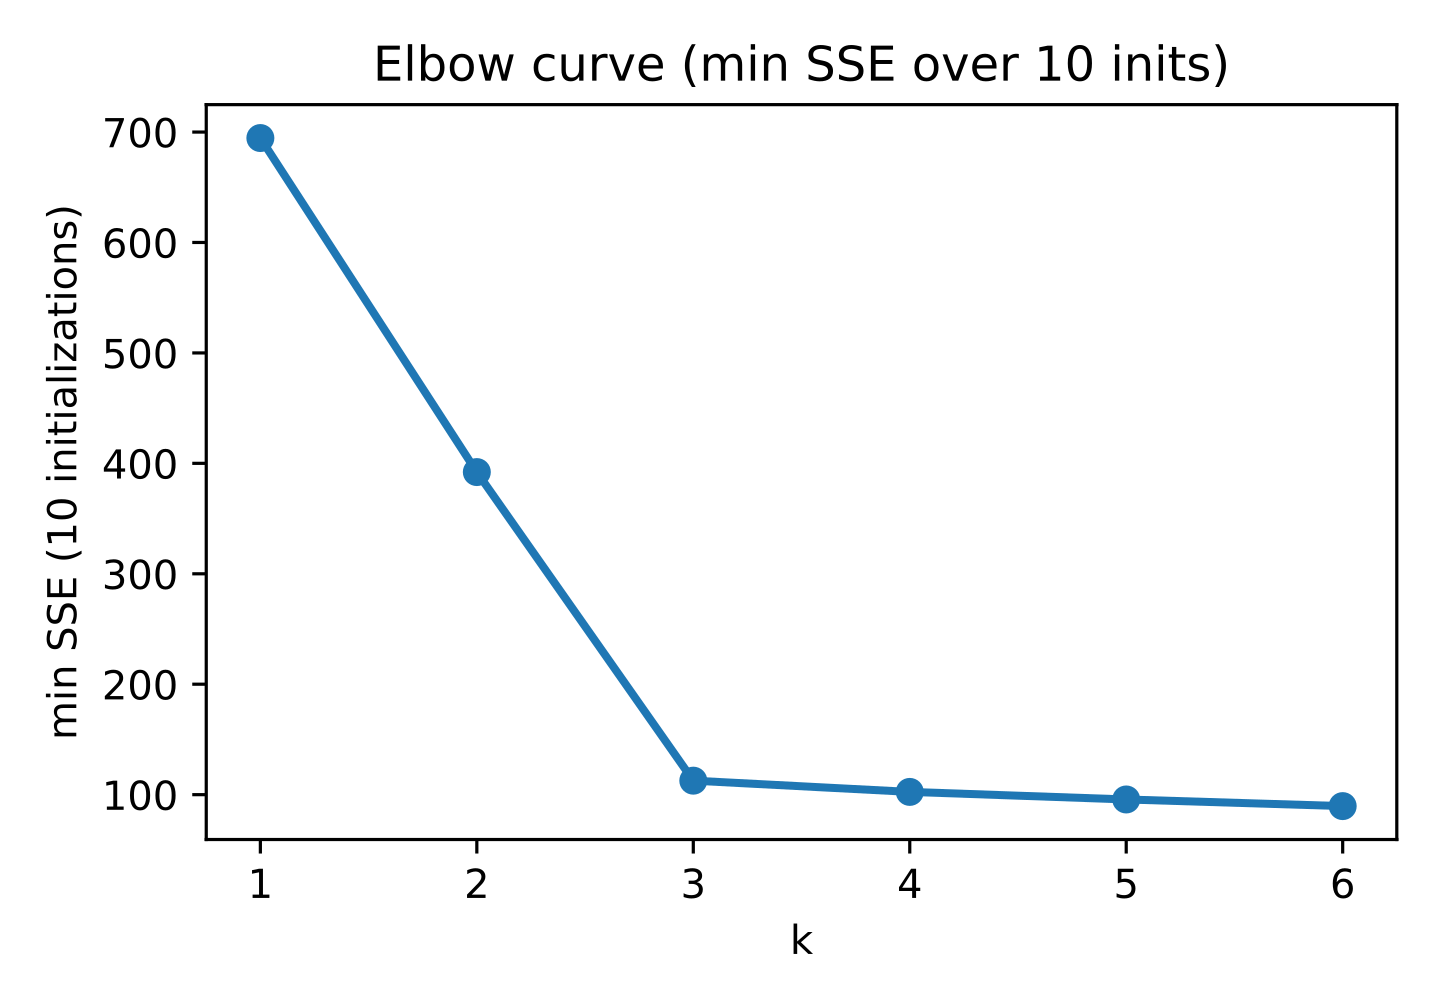
\includegraphics[width=\linewidth]{ch04_kmeans_elbow.png}
    \end{column}
    \begin{column}{0.43\textwidth}
      \begin{itemize}\small
        \item 그래프를 그리면 $k=3$에서 \textbf{각도가 꺾이는}
          ``팔꿈치''가 정확히 여기에 옴
        \item \textbf{솔직히}: 엘보우는 항상 이렇게 선명한 각도를
          만들지 않음 --- 덩어리가 서로 가깝거나 크기가 비슷하면
          곡선이 완만해져 ``여기다!''를 확신하기 어려움
      \end{itemize}
      \vskip0.4em
      \textbf{완만할 때의 대응}:
      \begin{itemize}\small
        \item (i) 여러 초기화로 SSE의 \textbf{분포} 보기
        \item (ii) \kb{실루엣(silhouette) 점수} 등 다른 지표로
          교차 검증
      \end{itemize}
    \end{column}
  \end{columns}
\end{frame}

\begin{frame}{절대 하지 말 것: 최소 SSE로 k 고르기}
  \begin{alertblock}{함정}
    SSE는 $k$가 커질수록 \textbf{항상} 줄어든다(클러스터가
    하나 더 생기면 오차가 작아지는 건 당연한 결과).
    ``SSE가 가장 작은 $k$''를 고르면 \textbf{$k=n$}(각 점을
    개별 클러스터로)이 되어버린다.
  \end{alertblock}
  \vskip0.8em
  \begin{block}{원리}
    기준은 항상 \textbf{``감소폭이 급격히 줄어드는 지점''}이다.
    \begin{itemize}\small
      \item 엘보우 = \textbf{눈}으로 그 꺾임을 찾는 방법
      \item 4.4절 \kb{BIC} = 같은 결정을 \textbf{하나의 숫자}로
        내리는 \textbf{원리 있는 버전}
      \item 이 함정은 4.4절에서 ``likelihood로 $K$를 고르면
        $K=m$이 이긴다''는 모습으로 \textbf{다시} 등장
    \end{itemize}
  \end{block}
\end{frame}

\begin{frame}{손으로 한 번: 두 번의 반복을 따라가기}
  점 4개 $(1,1), (1,2), (8,8), (9,8)$, $k=2$,
  초기 $c_0=(1,2)$, $c_1=(8,8)$.
  \vskip0.4em
  \kb{1회차 할당}:
  \begin{itemize}\small
    \item $(1,1)$: $c_0$까지 1, $c_1$까지 $\approx9.9$ $\to$ $c_0$
    \item $(1,2)$: $c_0$과 같은 점(거리 0) $\to$ $c_0$
    \item $(8,8)$: $c_1$과 같은 점 $\to$ $c_1$
    \item $(9,8)$: $c_1$까지 1 $\to$ $c_1$
  \end{itemize}
  \kb{1회차 갱신}(각 그룹의 평균):
  \[
  c_0 \leftarrow \left(\tfrac{1+1}{2}, \tfrac{1+2}{2}\right) = (1,\, 1.5),
  \qquad
  c_1 \leftarrow \left(\tfrac{8+9}{2}, \tfrac{8+8}{2}\right) = (8.5,\, 8)
  \]
  \kb{2회차}: 새 중심점 $(1, 1.5), (8.5, 8)$으로 다시 할당 $\to$
  네 점의 소속이 1회차와 \textbf{정확히 동일} $\Rightarrow$
  \textbf{수렴} 판단, 멈춤. 최종 중심점 $(1, 1.5), (8.5, 8)$.
  \vskip0.4em
  {\footnotesize 수학적으로도: 초기 $J=2.0$(각 점 기여 1) $\to$
  갱신 후 $J=1.0$(기여 0.25로 감소) --- 단조감소, 2회차에 할당
  변경 없어 멈춤.}
\end{frame}

\begin{frame}{자주 하는 실수: 초기화의 영향을 무시}
  k-means는 \textbf{볼록하지 않은}(non-convex) 최적화 문제 ---
  경사하강법처럼 초기 중심점을 어디서 시작하느냐에 따라
  \textbf{다른 지역 최적해}에 도달할 수 있다.
  \vskip0.6em
  \begin{itemize}
    \item 초기 중심점 두 개가 우연히 \textbf{같은 덩어리 안에
      가깝게} 잡히면: 그 덩어리를 둘로 \textbf{잘못 쪼개고}
      다른 덩어리 하나를 \textbf{통째로 놓쳐} 수렴
    \item 실전에서 흔히 하는 실수: \texttt{kmeans(X, k)}를
      \textbf{딱 한 번만} 돌리고 결과를 그대로 믿음
  \end{itemize}
  \vskip0.6em
  \begin{block}{표준 대응}
    \begin{enumerate}\small
      \item 서로 다른 무작위 초기화로 \textbf{여러 번}(예: 10회)
        돌려서, 그중 \textbf{클러스터 내 분산이 가장 작은}
        결과를 채택 (\texttt{sklearn.cluster.KMeans}의 기본
        \texttt{n\_init}이 정확히 이 역할)
      \item 또는 \kb{k-means++}처럼 서로 멀리 떨어진 점을
        우선적으로 고르는 \textbf{똑똑한 초기화}로 나쁜
        지역최적해에 빠질 확률 자체를 크게 줄임
    \end{enumerate}
  \end{block}
\end{frame}

\begin{frame}{실험: 60번 중 1번이 크게 망가진다}
  3-블롭 데이터(각 50점, 총 150점), 무작위 3점 초기화로
  k-means \textbf{60번} 돌려 수렴한 SSE 기록:
  \small
  \begin{tabular}{@{}ll@{}}
    \toprule
    초기화 & SSE \\
    \midrule
    59회 & 258.4 (\textbf{정답 구조}: 3개 덩어리 각각) \\
    1번 (실패) & \textbf{1845.3} (정답의 \textbf{7.1배}) \\
    \bottomrule
  \end{tabular}
  \vskip1em
  실패 사례의 초기 중심점 $(1.08, 2.50), (7.73, 9.01),
  (0.80, 2.49)$ --- \textbf{첫째와 셋째가 왼쪽 덩어리 안에 가깝게}
  잡힘. 1회차에 왼쪽 50점 중 43점이 첫 중심점, 7점이 세 번째에
  배정, 오른쪽 두 덩어리는 중간 중심점 \textbf{하나에 통째로
  흡수}. 알고리즘은 이 ``잘못된 분할''이 이미 \textbf{지역적으로
  일관}되므로(각 점은 자기 중심으로 볼 때 여전히 가장 가깝다)
  여기서 멈추는 게 최적이라고 판단 --- 4회차 만에 \textbf{잘못된
  수렴}. 최종 크기 [41, 100, 9].
  \vskip0.4em
  60번 중 1번(약 1.7\%) --- \textbf{데이터가 더 조밀하고 덩어리
  사이 간격이 좁아질수록 이 확률은 훨씬 높아짐}.
  ``한 번만 돌려도 대부분 맞으니까''는 \textbf{위험한 베팅}.
\end{frame}

\begin{frame}{똑똑한 초기화: k-means++}
  무작위 초기화의 결함 구조: $k$개 중심점을 데이터에서
  \textbf{독립적으로} 무작위로 뽑으면, 여러 중심점이
  \textbf{같은 좁은 영역에 몰리는} 가능성을 스스로 만듦.
  k-means++는 이 결함을 정면으로 고친다:
  \vskip0.4em
  \begin{enumerate}\small
    \item 첫 중심점: 데이터에서 \textbf{균등 무작위}
    \item 각 점 $x$에 대해 이미 고른 중심점까지의 \textbf{최소
      거리} $D(x)$ 계산 $\to$ \textbf{$D(x)^2$에 비례하는 확률}로
      다음 중심점 선택
    \item $k$개 다 고를 때까지 2 반복
  \end{enumerate}
  \vskip0.6em
  핵심: ``가장 가까운 중심점에서 \textbf{멀리} 있는 점을 더 높은
  확률로 고른다'' --- 첫 중심점이 왼쪽 덩어리에 놓이면 두 번째는
  오른쪽 덩어리에서 상대적으로 높은 확률로 추첨 $\to$
  \textbf{같은 덩어리에 두 중심점이 몰리는 상황을 구조적으로
  막음}.
  \vskip0.4em
  왜 \textbf{제곱}? Arthur \& Vassilvitskii(2007)의
  k-means++ 논문: $D(x)^2$-비례 선택을 쓸 때, 최종 분할의 SSE가
  \textbf{기댓값 기준으로} 최적 분할 SSE의 $O(\log k)$배
  이내(원논문 bound $8\ln k + 7$배)에 머문다는
  \textbf{증명 가능한 근사 보장} --- 단순 무작위에는 없는 성질.
\end{frame}

\begin{frame}{k-means++ vs 단순 무작위}
  같은 3-블롭 데이터, 초기화 20회 비교:
  \small
  \begin{tabular}{@{}ll@{}}
    \toprule
    초기화 & SSE 범위 (20회) \\
    \midrule
    단순 무작위 & 258.4 $\sim$ 2210.7 (\textbf{최소한 1$\sim$2회
                  크게 이탈}) \\
    k-means++ & 258.4 $\sim$ 258.4 (\textbf{모두 동일}) \\
    \bottomrule
  \end{tabular}
  \vskip1em
  \begin{itemize}
    \item k-means++가 ``\textbf{무작위성을 없애주는}'' 게
      아니라, ``\textbf{나쁜 무작위성의 가능성을 크게 줄여주는}''
      것 --- 이론적으로는 여전히 지역 최소해에 빠질 수 있다
  \end{itemize}
  \vskip0.6em
  \begin{block}{실전 표준 조합}
    \textbf{k-means++ 초기화 + \texttt{n\_init}회 반복} 두 가지를
    \textbf{함께}. \texttt{sklearn.cluster.KMeans}의 기본값이
    \texttt{init="k-means++"}, \texttt{n\_init=10}인 이유가
    바로 이것.
  \end{block}
\end{frame}

\begin{frame}{k-means의 한계: ``원형 덩어리'' 전제}
  거리로 가장 자연스러운 분할을 잘 \textbf{하는 반면}, 데이터가
  \textbf{원형(볼록) 덩어리}라는 전제에 묶여 있다:
  \vskip0.6em
  \small
  \begin{itemize}
    \item \kb{볼록하지 않은 구조를 못 그림} --- 마주 보는 두
      반달을 각 반달을 \textbf{반으로 자르는 직선 경계}(두
      중심점의 수직이등분선)로 잘게 쪼개 SSE를 더 작게 만든다고
      판단할 수 있음. 경계가 \textbf{항상 직선}이라 곡선을 따라
      흐르는 구조를 표현할 방법이 구조적으로 없음
    \item \kb{아웃라이어에 약함} --- 중심점이 \textbf{산술
      평균}이라 멀리 떨어진 점 하나가 있어도 그쪽으로 끌려감.
      중앙값으로 대신하면 완화되나, ``평균이 SSE를 최소화하는
      점''이라는 수학이 더 이상 성립하지 않음
    \item \kb{모든 클러스터를 ``같은 크기/형상''으로 취급} ---
      표현은 \textbf{중심점 하나}(위치 벡터)뿐. 넓고 좁은지,
      타원형인지 담을 수 없음 $\to$ \textbf{4.4절 GMM}이 바로
      이 한계를 고침
    \item \kb{$k$를 미리 알아야 함} (앞 엘보우 섹션)
  \end{itemize}
\end{frame}

\begin{frame}{유명한 사례: 두 번 발견된 알고리즘}
  k-means의 기원 = ML 역사에서 \textbf{``동시 독립
  발견''}(simultaneous discovery)의 대표 사례:
  \vskip0.6em
  \begin{columns}[T]
    \begin{column}{0.48\textwidth}
      \kb{로이드 (Lloyd, 1957)}
      \begin{itemize}\small
        \item 벨 연구소, \textbf{PCM}(상용 전화 신호를 디지털로
          변환)의 양자화 문제 연구 중 발명
        \item 정식 논문 전에 \textbf{내부 보고서}로만 머물러 있었음
      \end{itemize}
    \end{column}
    \begin{column}{0.48\textwidth}
      \kb{매퀸 (MacQueen, 1967)}
      \begin{itemize}\small
        \item 스탠퍼드, \textbf{클러스터링} 문제에서
          \textbf{독립적으로} 같은 알고리즘 재발명
        \item ``k-means''라는 \textbf{이름}과 함께 발표
        \item 로이드가 훨씬 먼저였다는 사실이 알려지기까지 꽤
          오래 걸림
      \end{itemize}
    \end{column}
  \end{columns}
  \vskip0.6em
  두 발견은 \textbf{문제가 달랐는데}(신호 양자화 vs 데이터
  클러스터링), 핵심 구조(\textbf{거리로 가장 가까운 대표에 할당
  $\to$ 대표 재계산})가 정확히 같았다.
  \vskip0.4em
  \begin{block}{교훈}
    \textbf{``거리 기반 반복 재할당''은 특정 도메인의 트릭이
    아니라, 거리 함수 위에서 자연스러운 최적화 구조 그
    자체} --- 같은 패턴이 서로 다른 문제에서 반복 등장하는 이유.
  \end{block}
\end{frame}

\begin{frame}{kNN과의 차이 --- 그리고 단순함의 가치}
  \begin{columns}[T]
    \begin{column}{0.5\textwidth}
      \kb{kNN}(게으름, lazy)
      \begin{itemize}\small
        \item 예측할 때마다 \textbf{그때그때} 거리 재기
        \item 거리 계산이 \textbf{예측 시점}에 몰려 있음
      \end{itemize}
    \end{column}
    \begin{column}{0.5\textwidth}
      \kb{k-means}
      \begin{itemize}\small
        \item 중심점이 \textbf{수렴할 때까지} 데이터를
          반복적으로 훑음
        \item 거리 계산이 ``\textbf{학습} 단계''에 몰려 있음
          $\Rightarrow$ 오히려 \textbf{선형회귀 같은 파라미터
          학습} 쪽에 더 가깝다
        \item \textbf{라벨이 없다는 것만} 지도학습과 다름
      \end{itemize}
    \end{column}
  \end{columns}
  \vskip0.8em
  \begin{block}{단순함이 곧 약점이 아니다}
    kNN과 k-means 둘 다 모델이 ``무엇을 학습했는지''를 설명해주는
    복잡한 이론이 없지만, \textbf{바로 그 단순함}(순전히 거리
    계산) 덕분에 \textbf{언제, 왜 실패하는지도 수식으로
    정확히} 짚어낼 수 있다.
  \end{block}
\end{frame}

\begin{frame}{자주 묻는 질문 (4.3)}
  \small
  \begin{itemize}
    \item \textbf{Q. k-means가 항상 수렴하나요?}
      그렇다 --- 매 반복마다 SSE가 절대 늘지 않고 $0$ 이상이므로
      \textbf{유한한 시간 안에} 수렴이 보장. 다만
      \textbf{어디로} 수렴하는지(전역 vs 나쁜 지역최적해)는
      보장되지 않음 = ``자주 하는 실수''의 핵심
    \item \textbf{Q. $k$를 몰라도 쓸 수 있나요?}
      k-means 자체는 $k$를 \textbf{미리} 정해야 함.
      $k$를 데이터로부터 자동으로 원하면: 엘보우로 여러 $k$를
      비교하거나, 4.4절 EM/GMM처럼 각 클러스터의 ``적합도''를
      \textbf{확률적으로} 비교할 수 있는 모델로 넘어가기
    \item \textbf{Q. 왜 항상 ``원형'' 덩어리만 찾나요?}
      \textbf{구조적으로} 결정됨 --- 두 클러스터의 경계는
      ``두 중심점까지 거리가 같은 점들의 집합''이고, 2차원에선
      \textbf{직선}(수직이등분선) $\Rightarrow$ 각 클러스터 영역은
      반드시 \textbf{볼록} 다각형(보로노이 셀). 반달·고리 모양
      경계를 그릴 \textbf{자유 자체가 모델 안에 없음} ---
      파라미터 튜닝으로 극복할 수 없는 \textbf{구조적} 한계
    \item \textbf{Q. 클러스터가 비어(멤버 0)질 수 있나요?}
      이론적으로 가능 --- 어떤 중심점도 어떤 점에게도 ``가장
      가까운''이 아닌 상황. \texttt{if cluster else
      centroids[i]} 분기가 바로 이걸 막음(빈 클러스터의
      ``평균''은 정의되지 않음 $\to$ 중심점 유지가 관례)
    \item \textbf{Q. 차원이 높으면 k-means도 안 쓰나요?}
      4.2절의 차원의 저주가 \textbf{그대로} 적용 --- ``가장
      가까운 중심점'' 구분이 점점 무뎌짐. 실무 표준:
      \textbf{Ch.\,14 PCA로 차원 축소}한 뒤 2$\sim$3차원 공간에서
      클러스터링
  \end{itemize}
\end{frame}

% ============================================================
\section{4.4 GMM, EM 알고리즘, 그리고 LDA}

\begin{frame}{닭이 먼저냐 달걀이 먼저냐: 잠재변수 문제}
  4.3절 k-means는 각 점을 \textbf{딱 하나의} 클러스터에 배정
  (\kb{하드 할당}). 실제 데이터는 경계가 \textbf{모호}한 경우가
  많다 --- 어떤 점은 ``A에 60\%, B에 40\%'' 속한다고 보는 게 더
  자연스러울 수 있다.
  \vskip0.8em
  \begin{itemize}
    \item \kb{가우시안 혼합모델(GMM)}: 각 클러스터를
      \textbf{정규분포}로 표현(Ch.\,3 GDA와 같은 가정)하고,
      각 점이 어느 클러스터에서 왔는지를 \textbf{확률}로
      표현(소프트 할당)
    \item 문제는 각 점의 \textbf{진짜} 클러스터 $z$가 데이터에
      \textbf{관측되지 않음}(\kb{잠재변수}, latent variable)
  \end{itemize}
  \vskip0.6em
  \begin{block}{순환}
    \begin{itemize}\small
      \item $z$(진짜 클러스터)를 \textbf{안다면} $\to$ 각
        클러스터의 평균·분산 구하기 \textbf{쉬움}(GDA처럼)
      \item 평균·분산을 \textbf{안다면} $\to$ 각 점의
        \textbf{사후확률} $z$ 구하기 \textbf{쉬움}(베이즈 정리)
      \item \textbf{둘 다 모른다} = 닭 vs 달걀의 순환
    \end{itemize}
  \end{block}
  EM은 이 순환을 \textbf{반복}으로 풀어낸다: 하나를 (아무 값으로)
  고정 $\to$ 다른 하나를 구함 $\to$ 그걸로 다시 처음 것을 고침,
  \textbf{값이 더 이상 바뀌지 않을 때까지}.
\end{frame}

\begin{frame}{유명한 사례: 절차의 이름이 곧 알고리즘 이름}
  1977년 통계학자 \kb{뎀스터(Dempster)·레어드(Laird)·루빈
  (Rubin)}가 잡지 \emph{JRSS-B}에 발표한
  ``\textbf{Maximum Likelihood from Incomplete Data via the EM
  Algorithm}'' --- 통계학에서 가장 많이 인용된 논문 중 하나.
  \vskip0.8em
  \begin{itemize}
    \item 놀랍게도 이 논문의 ``발명품''은 \textbf{전혀 새로운
      수학이 아님} --- E-step 계산(현재 파라미터에서의 사후확률)도,
      M-step 갱신 공식도 그 전부터 알려져 있었음
    \item 세 사람이 한 일은 \textbf{통합}: \kb{혼합모델 · 결측값 ·
      HMM · 양자화}처럼 겉보기엔 별개의 여러 통계 문제가
      \textbf{사실 전부 같은 구조}라는 것
      --- ``관측 안 된 변수가 있으면 M-step이 쉽고, 파라미터가
      주어지면 E-step이 쉽다''. 이 둘을 번갈아 돌리면
      \textbf{우도가 절대 줄지 않으니 반드시 수렴}
    \item ``\kb{EM}''이라는 이름 자체가 E-step과 M-step이라는
      \textbf{두 절차의 앞글자} 그대로 = 이 논문의 성격
  \end{itemize}
  \vskip0.6em
  k-means가 ``동시에 독립적으로 두 번 \textbf{발견}된'' 사례라면,
  EM은 그 \textbf{반대 방향}의 통합 사례 --- \textbf{여러
  알고리즘이 사실 하나였음을} 보인 사건. Ch.\,15(생성 모델)의
  ``관측되지 않은 구조가 데이터를 만든다''는 질문이 바로 이
  논문에서 하나의 알고리즘으로 정리되기 시작.
\end{frame}

\begin{frame}{GMM의 생성 과정}
  GMM을 ``\textbf{데이터가 만들어지는 과정}''으로 기술하면
  매우 단순하다:
  \vskip0.6em
  \begin{enumerate}
    \item \kb{라벨 뽑기}: $K$개 면의 \textbf{주사위}(카테고리
      분포)를 굴려 $z_i \in \{1, \dots, K\}$ 뽑기 --- 각 면의
      확률 $\pi_k$
    \item \kb{점 뽑기}: 뽑힌 클러스터 $z_i = k$의 정규분포
      $\mathcal{N}(\mu_k, \Sigma_k)$에서 점 $x_i$ 샘플링
  \end{enumerate}
  \vskip0.6em
  (1차원 예제에선 $\Sigma_k$가 스칼라 $\sigma_k^2$로 쓰인다.)
  \textbf{모수 세 종류}: 클러스터별 평균 $\mu_k$, 분산
  $\sigma_k^2$, \textbf{혼합비율} $\pi_k$ ($\sum_k \pi_k = 1$).
  \vskip0.6em
  이 모델이 정의하는 한 점의 likelihood:
  \[
  p(x) = \sum_{k=1}^{K} \pi_k \, \mathcal{N}(x; \mu_k, \sigma_k^2)
  \]
\end{frame}

\begin{frame}{왜 MLE로 바로 풀리지 않는가: 곱의 합}
  \begin{columns}[T]
    \begin{column}{0.48\textwidth}
      \kb{Ch.\,3 GDA / 나이브베이즈}
      \begin{itemize}\small
        \item ``\textbf{라벨이 주어지면}'' 파라미터별
          likelihood가 \textbf{곱의 합}으로 깔끔하게 풀림
        \item $\Rightarrow$ \textbf{닫힌 형태}의 MLE 공식 존재
      \end{itemize}
    \end{column}
    \begin{column}{0.48\textwidth}
      \kb{GMM}
      \begin{itemize}\small
        \item 라벨 $z$가 \textbf{관측되지 않아}
        \item 전체 likelihood =
          $\prod_i \big(\sum_k \pi_k \mathcal{N}(x_i;
          \mu_k, \sigma_k^2)\big)$
        \item = \textbf{곱의 합}
      \end{itemize}
    \end{column}
  \end{columns}
  \vskip0.8em
  \kq{합이 곱 안에 끼어 있으면 미분을 0으로 놓고 풀 수 있는
  구조가 아니다.}
  \vskip0.6em
  \begin{block}{EM의 본질}
    ``만약 $z$가 \textbf{알렸다면}''은 Ch.\,3 GDA와 \textbf{똑같이}
    닫힌 형태로 풀린다 --- EM은 이 \textbf{``만약''을 반복적으로
    실행}하는 알고리즘.
  \end{block}
\end{frame}

\begin{frame}{잠재변수 다이어그램}
  \begin{columns}[T]
    \begin{column}{0.55\textwidth}
      \centering
      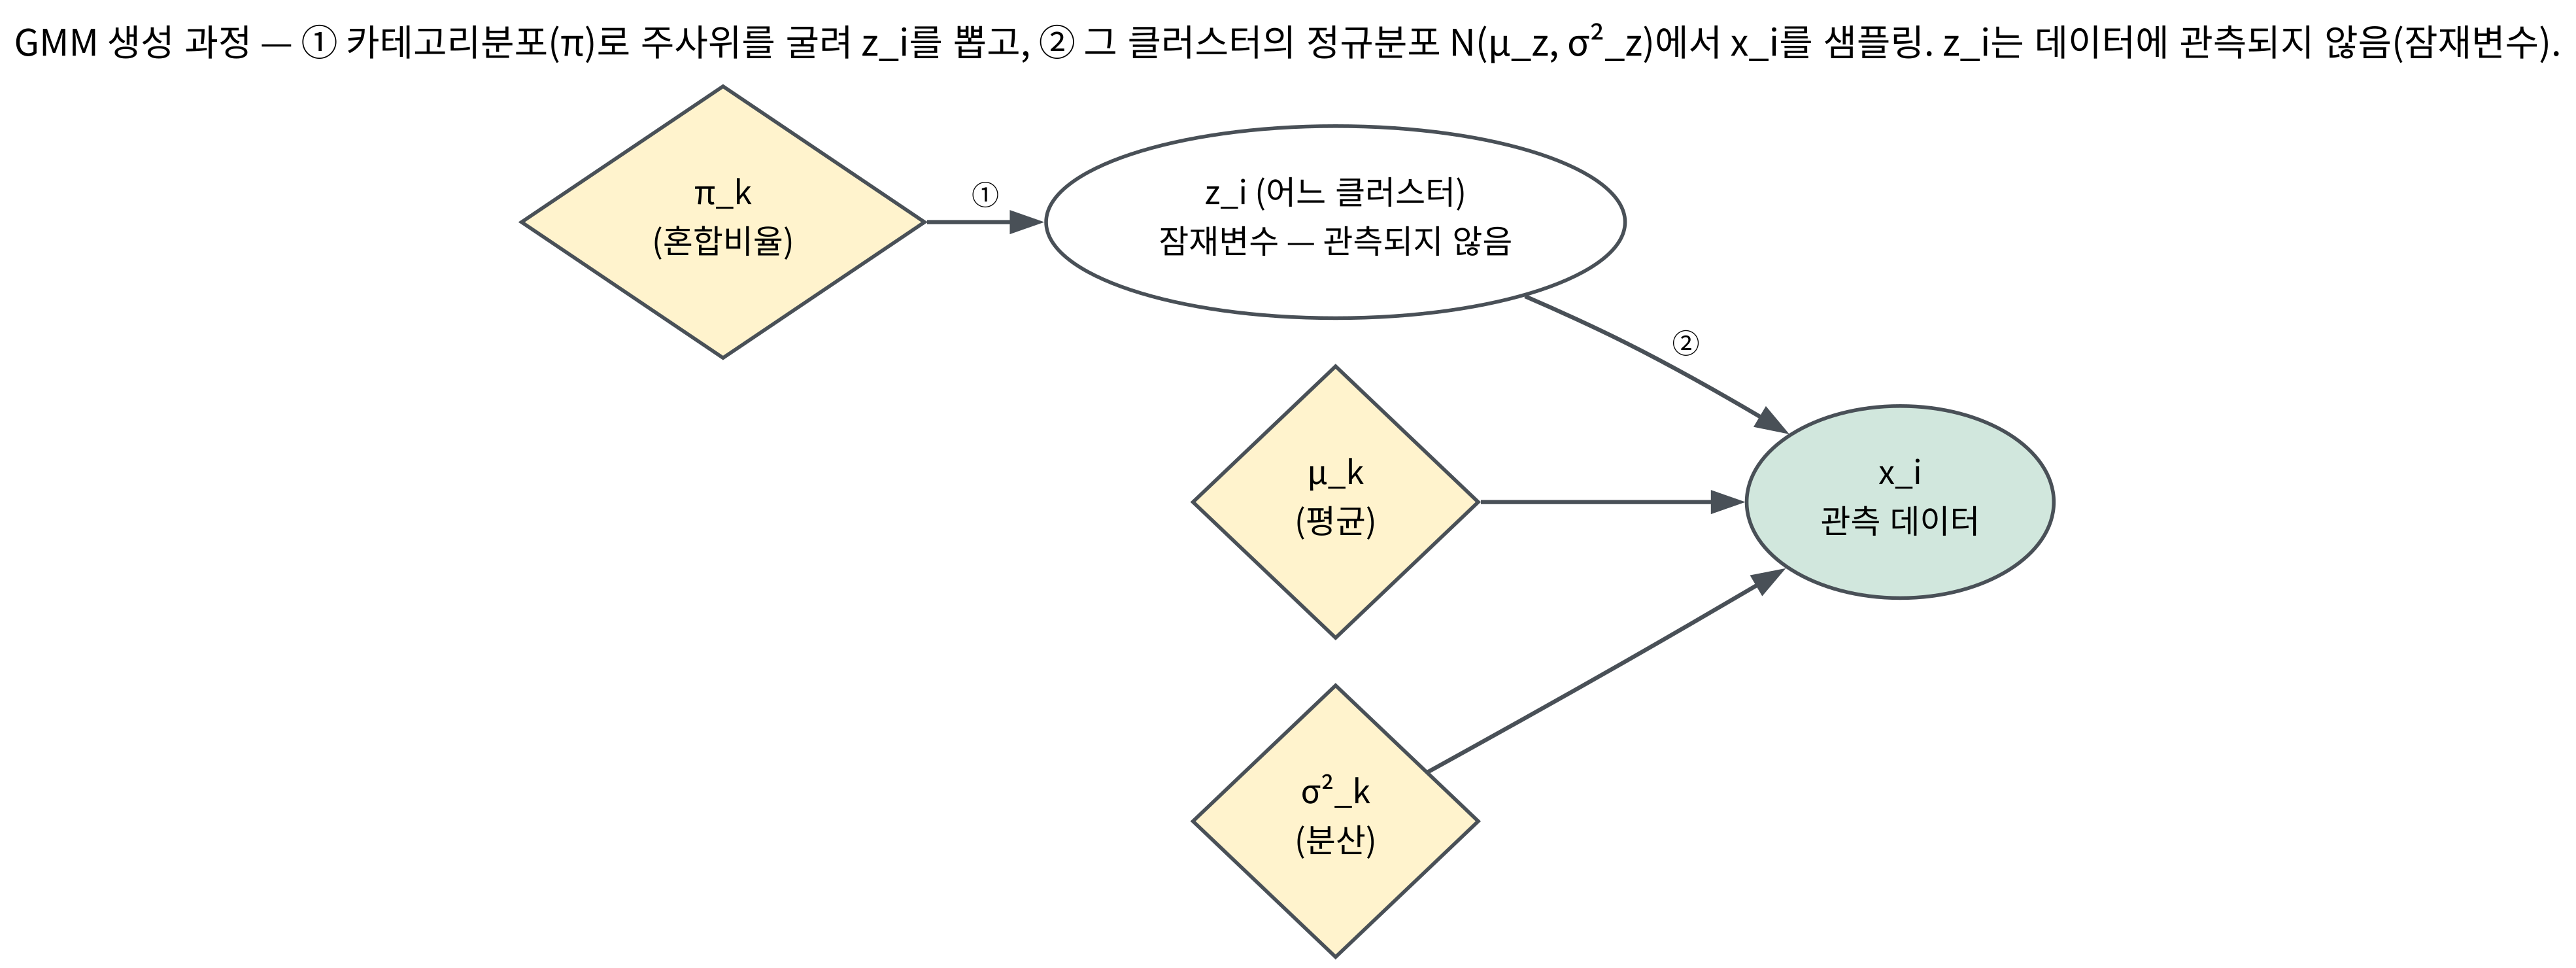
\includegraphics[width=\linewidth]{ch15_gmm_latent_var.png}
    \end{column}
    \begin{column}{0.43\textwidth}
      \begin{itemize}\small
        \item \textbf{마름모}($\pi_k, \mu_k, \sigma^2_k$) =
          \textbf{모수}
        \item \textbf{빈 원} $z_k$ = \textbf{관측되지 않는
          잠재변수}(어느 클러스터인지)
        \item \textbf{채워진 원} $x_i$ = \textbf{관측 데이터}
        \item $\pi_k$가 $z_k$를, $z_k$와 $(\mu_k, \sigma^2_k)$가
          $x_i$를 \textbf{만든다}
      \end{itemize}
      \vskip0.4em
      ``관측되지 않은 구조($z$)가 관측된 데이터($x$)를 만든다''
      --- Ch.\,15 생성 모델 전체가 이 그림의 변주.
    \end{column}
  \end{columns}
\end{frame}

\begin{frame}{EM 알고리즘: E-step}
  \kb{E-step (Expectation)} --- 현재 각 클러스터의 파라미터
  ($\mu_k, \sigma_k^2, \pi_k$)가 주어졌다고 가정하고, 각 데이터
  점 $x_i$가 클러스터 $k$에 속할 \textbf{사후확률}
  (\kb{책임값}, responsibility) $\gamma_{ik}$를 \textbf{베이즈
  정리}로 계산:
  \[
  \gamma_{ik} = P(z_i{=}k \mid x_i)
  = \frac{\pi_k \, \mathcal{N}(x_i; \mu_k, \sigma_k^2)}
         {\sum_{j} \pi_j \, \mathcal{N}(x_i; \mu_j, \sigma_j^2)}
  \]
  \begin{itemize}
    \item 분자: ``$k$번 클러스터가 $x_i$를 만들 확률''
      (선후확률, prior $\times$ likelihood)
    \item 분모: \textbf{모든} 클러스터 중 $x_i$를 만들 확률의
      합 $\Rightarrow$ $\gamma_{ik}$는 $0\sim1$의 \textbf{실수}
    \item $\sum_k \gamma_{ik} = 1$ (각 점은 모든 클러스터에
      확률 합 1로 분배됨)
  \end{itemize}
\end{frame}

\begin{frame}{EM 알고리즘: M-step}
  \kb{M-step (Maximization)} --- 방금 구한 책임값을
  \textbf{``가중치''}로 삼아, 각 클러스터의 파라미터를
  \textbf{다시 추정} --- $\gamma_{ik}$가 클수록 그 점이
  $\mu_k, \sigma_k^2$ 추정에 더 크게 기여:
  \[
  \mu_k = \frac{\sum_i \gamma_{ik} x_i}{\sum_i \gamma_{ik}},
  \qquad
  \sigma_k^2 = \frac{\sum_i \gamma_{ik}(x_i-\mu_k)^2}{\sum_i \gamma_{ik}},
  \qquad
  \pi_k = \frac{\sum_i \gamma_{ik}}{m}
  \]
  \vskip0.6em
  \begin{block}{한 번 더 천천히 보면 --- 정말 새 수식이 아님}
    ``라벨이 \textbf{전부 $k$}인 점들의 \textbf{평균·분산·
    비율}''(Ch.\,3의 \textbf{닫힌 형태 MLE})에서, 각 점의
    ``소속 여부''($0$ 또는 $1$)를 \textbf{책임값
    $\gamma_{ik}$}(0과 1 사이의 실수)로 \textbf{바꾼 것}뿐.
    E-step = ``\textbf{하드 라벨 대신 소프트 라벨을 채워넣는}''
    단계, M-step = ``\textbf{소프트 라벨이 주어졌을 때의 닫힌
    형태 MLE}'' --- \textbf{EM의 전부가 이 한 문장}.
  \end{block}
\end{frame}

\begin{frame}[fragile]{em\_step 코드 (1차원)}
\begin{lstlisting}
import math

def gaussian_pdf(x, mu, sigma):
    return (1 / (sigma * math.sqrt(2 * math.pi))) * \
           math.exp(-((x - mu) ** 2) / (2 * sigma ** 2))

def em_step(data, means, sigmas, weights):
    K, n = len(means), len(data)
    # E-step: 책임값(responsibility) 계산
    resp = []
    for x in data:
        probs = [weights[k] * gaussian_pdf(x, means[k], sigmas[k])
                 for k in range(K)]
        total = sum(probs)
        resp.append([p / total for p in probs])
    # M-step: 책임값으로 가중평균한 파라미터 재추정
    Nk = [sum(resp[i][k] for i in range(n)) for k in range(K)]
    new_means = [sum(resp[i][k] * data[i] for i in range(n)) / Nk[k]
                 for k in range(K)]
    new_sigmas = [math.sqrt(sum(resp[i][k] * (data[i] - new_means[k]) ** 2
                                for i in range(n)) / Nk[k])
                  for k in range(K)]
    new_weights = [Nk[k] / n for k in range(K)]
    return new_means, new_sigmas, new_weights
\end{lstlisting}
  {\footnotesize 한 라운드의 E-step + M-step. 이걸 ``변화가
  멈출 때까지'' 반복하면 EM 완성.}
\end{frame}

\begin{frame}{왜 우도가 항상 증가하는가: 옌센 부등식 (1)}
  ``E-step $\to$ M-step 반복하면 수렴한다''를 \textbf{그대로
  믿지 말자} --- *왜* 우도가 매 반복마다 절대 줄지 않는지
  \textbf{4줄}이면 보인다. 핵심은 \kb{ELBO}(Evidence Lower
  BOund) --- 이 이름은 Ch.\,15.1절에서 다시 만난다.
  \vskip0.6em
  하나의 점 $x$에 대해, $\gamma$를 $z$ 위의 \textbf{아무}
  확률분포라고 놓고:
  \[
  p(x) = \sum_{k} p(x, z{=}k)
  = \sum_{k} \gamma_k \frac{p(x, z{=}k)}{\gamma_k}
  = \mathbb{E}_{z \sim \gamma}\!\left[\frac{p(x, z)}{\gamma(z)}\right]
  \]
  \kb{$\log$은 오목함수}(concave) $\Rightarrow$
  \kb{옌센 부등식} $\log \mathbb{E}[X] \ge \mathbb{E}[\log X]$
  적용:
\end{frame}

\begin{frame}{왜 우도가 항상 증가하는가: 옌센 부등식 (2)}
  \[
  \log p(x) \ge \mathbb{E}_{z \sim \gamma}[\log p(x, z)]
  - \mathbb{E}_{z \sim \gamma}[\log \gamma(z)]
  \;\; \stackrel{\text{def}}{=} \;\; \mathcal{F}(\theta, \gamma)
  \]
  우변 $\mathcal{F}(\theta, \gamma)$가 \textbf{우도의 하한}.
  \textbf{등호가 성립하는 조건}: $\frac{p(x,z)}{\gamma(z)}$가
  $z$에 대해 \textbf{상수}, 즉 $\gamma$가 \textbf{진짜
  사후확률} $p(z|x)$인 경우 --- \textbf{바로 이 조건이 EM의
  설계 원리}.
  \vskip0.6em
  EM의 두 단계를 이 \textbf{하한}으로 읽으면:
  \begin{itemize}\small
    \item \kb{E-step}: $\gamma$를 \textbf{현재 파라미터
      $\theta_{\text{old}}$에서의 진짜 사후확률}로 잡음
      $\Rightarrow$ 등호가 성립해서
      $\mathcal{F}(\theta_{\text{old}}, \gamma) = \log
      p(x; \theta_{\text{old}})$ (하한이 \textbf{뚫리지 않는
      정도로 꽉 조인} 상태)
    \item \kb{M-step}: $\gamma$를 \textbf{고정}하고 $\theta$를
      $\mathcal{F}$를 최대화하도록 갱신 $\Rightarrow$
      $\mathcal{F}(\theta_{\text{new}}, \gamma) \ge
      \mathcal{F}(\theta_{\text{old}}, \gamma)$
  \end{itemize}
  두 걸을 합치면:
  \[
  \log p(x; \theta_{\text{new}}) \ge \mathcal{F}(\theta_{\text{new}}, \gamma)
  \ge \mathcal{F}(\theta_{\text{old}}, \gamma)
  = \log p(x; \theta_{\text{old}})
  \]
  \kq{우도가 매 반복마다 절대 줄지 않는다.}
  \vskip0.4em
  \textbf{6개 데이터로 실제로 확인}($m=6$,
  $[1.0,1.5,0.8,9.2,10.1,9.8]$, 초기 $\mu=[2,8],\sigma=[1,1],
  \pi=[0.5,0.5]$): log-likelihood가
  $-15.56 \to -6.05 \to -6.05$(2회차에 \textbf{멈춤}) ---
  \textbf{단조증가는 성립}하지만 도달한 점이 \textbf{전역
  최적해}라는 보장은 이 논증 어디에도 없음.
  \vskip0.4em
  Ch.\,15.1절 \kb{VAE}는 ``E-step의 사후확률을 정확히 계산할
  수 없을 때(연속 무한한 잠재변수) 이 하한을 \textbf{신경망}
  $q_\phi(z|x)$로 근사해서 \textbf{역전파}로 올린다''는
  알고리즘 --- EM과 VAE는 \textbf{같은 부등식의 두 실행
  전략}.
\end{frame}

\begin{frame}{2차원 GMM: 공분산 행렬 $\Sigma_k$}
  \begin{columns}[T]
    \begin{column}{0.55\textwidth}
      1차원에선 $\mu_k, \sigma_k^2$가 스칼라였지만 $d$차원에선
      $\mu_k \in \mathbb{R}^d$, $\Sigma_k \in \mathbb{R}^{d \times
      d}$(\kb{공분산 행렬}). E-step은 \textbf{그대로}, M-step은
      \textbf{가중 공분산}만 추가:
      \[
      \Sigma_k = \frac{\sum_i \gamma_{ik}(x_i - \mu_k)(x_i - \mu_k)^{\mathsf{T}}}
                     {\sum_i \gamma_{ik}}
      \]
      이 $\Sigma_k$가 \textbf{GMM이 k-means보다 표현력이 많은
      정체} --- k-means는 \textbf{위치}($\mu_k$) 하나뿐(경계
      \textbf{항상 직선}, ``동일한 크기의 원'')인데, $\Sigma_k$는
      (i) \textbf{크기}, (ii) \textbf{타원형 모양}, (iii)
      \textbf{기울어진(비대각) 형상}을 \textbf{모두} 표현. 결정경계
      도 ``두 정규분포의 \textbf{밀도비가 1인 곡선}'' $\Rightarrow$
      직선이 아닌 \textbf{타원호}.
    \end{column}
    \begin{column}{0.43\textwidth}
      \centering
      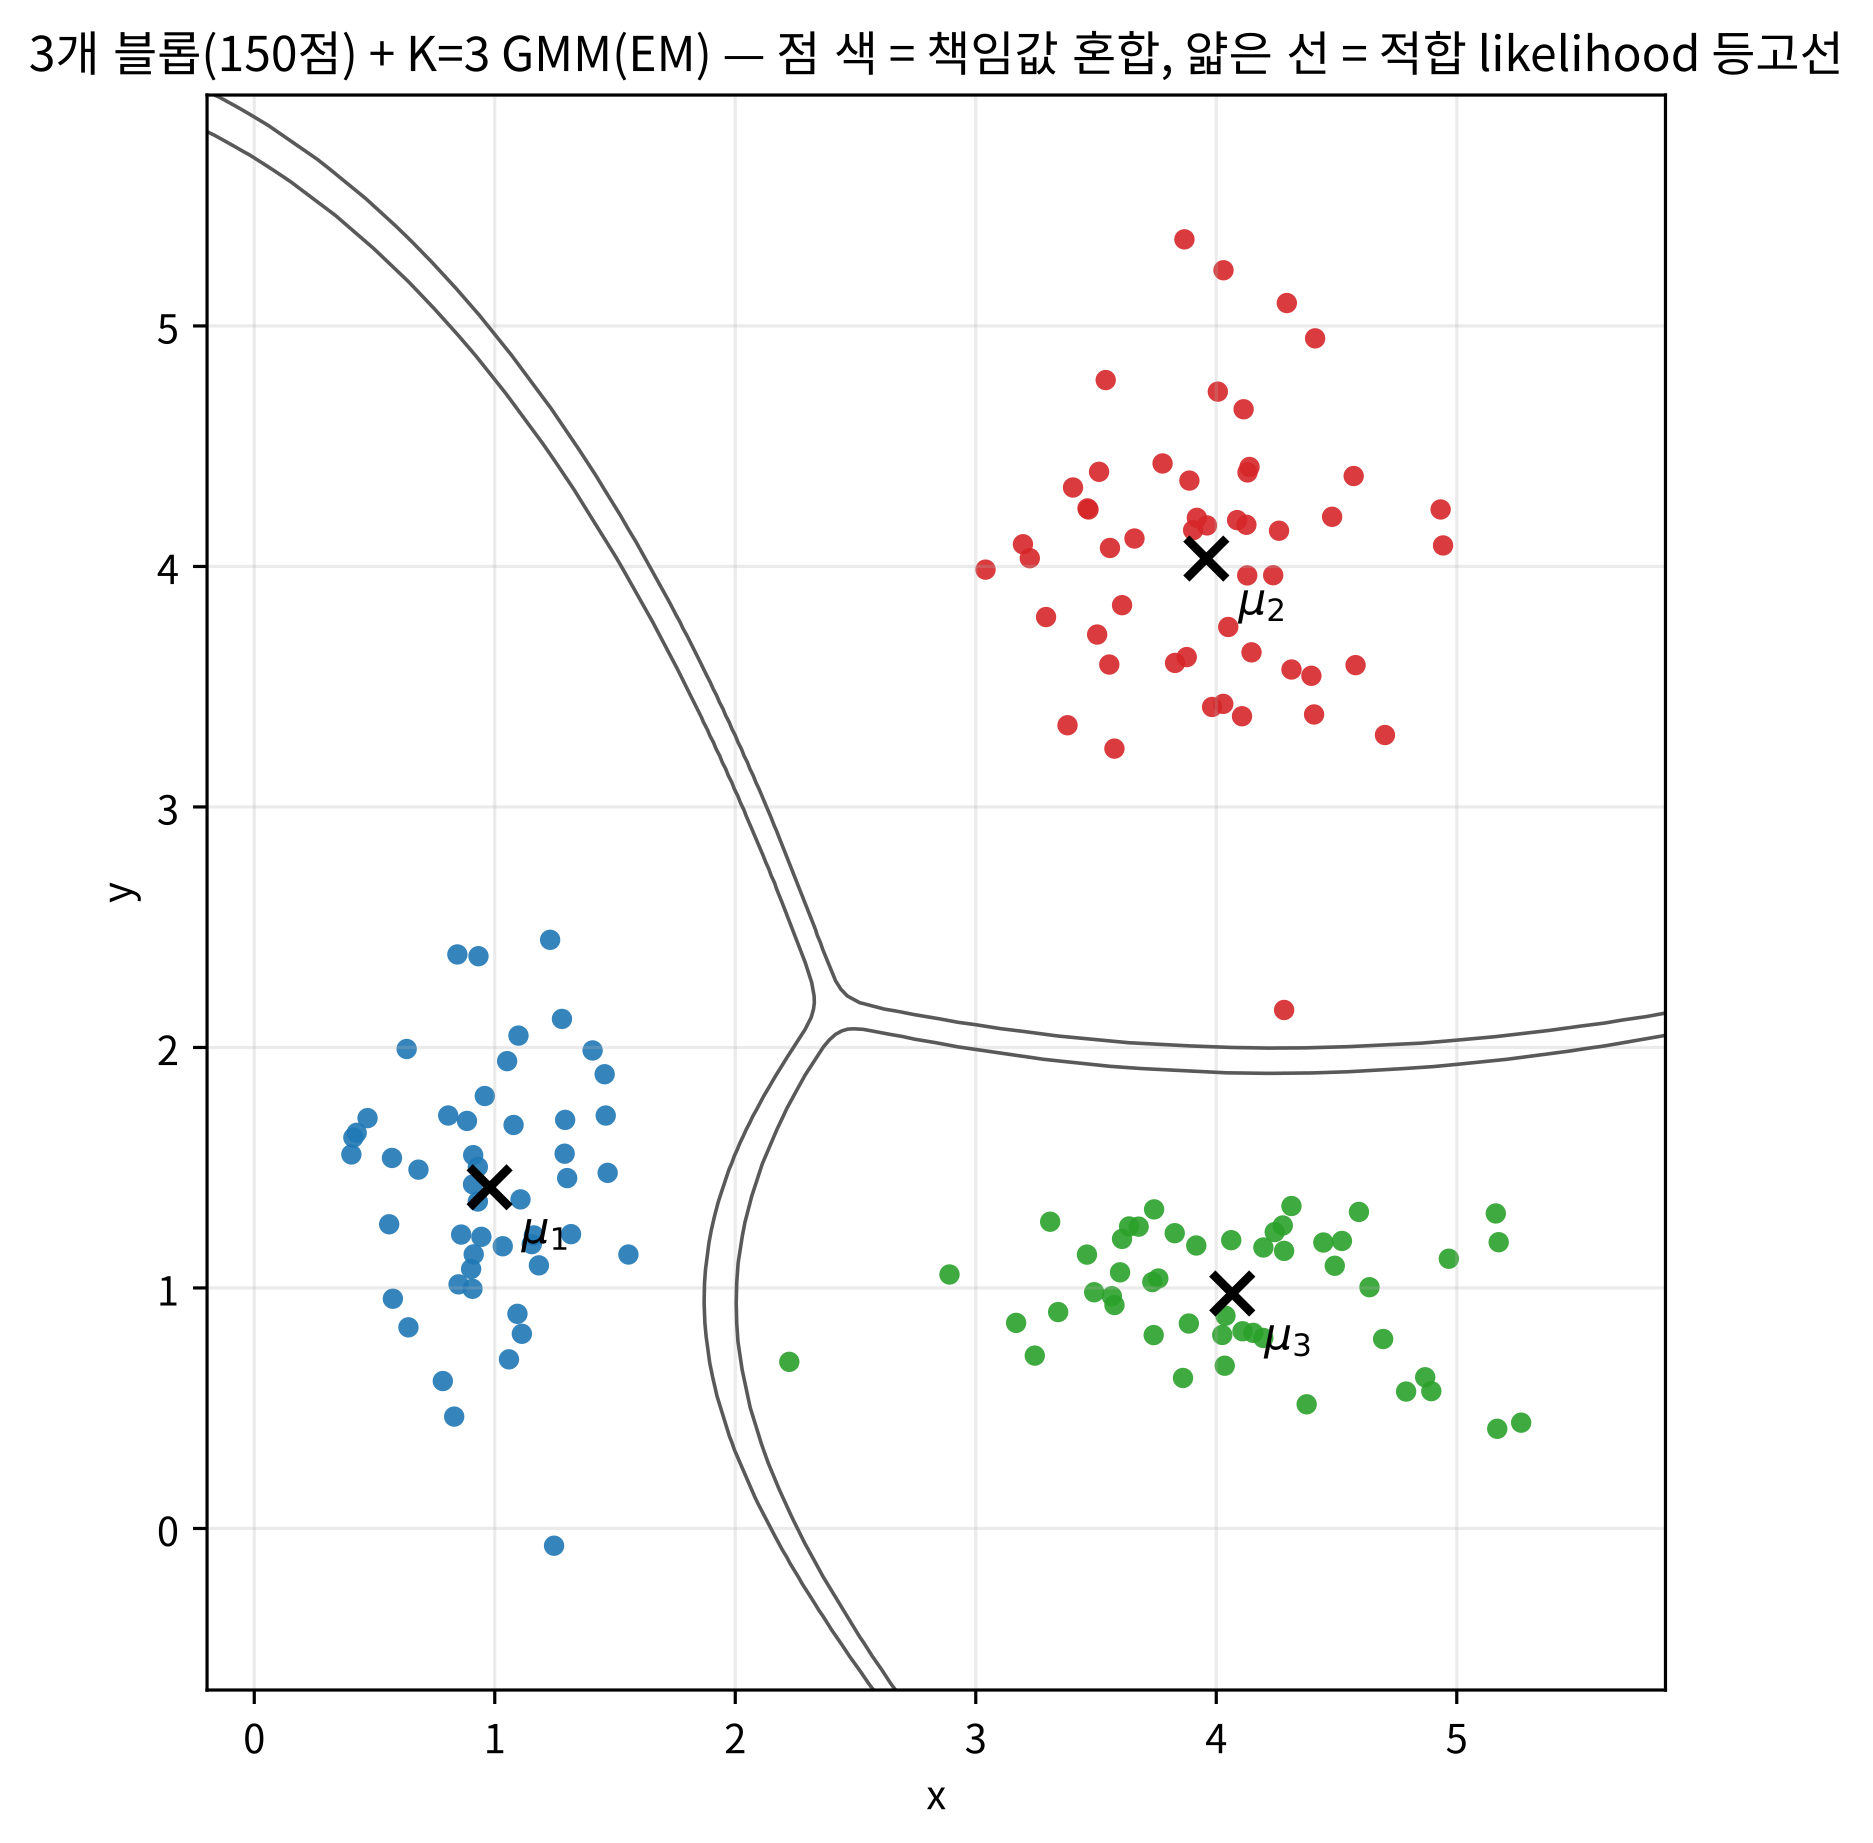
\includegraphics[width=\linewidth]{ch15_gmm_contour.png}
      \vskip0.4em
      {\footnotesize 3개 블롭(각 50점)에 $K=3$ GMM을 EM으로
      학습. 점 색=\textbf{책임값}, 등고선=likelihood. 왼쪽은
      \textbf{길쭉한 타원}, 위쪽은 \textbf{원}.}
    \end{column}
  \end{columns}
  \vskip0.4em
  \begin{block}{k-means와의 가장 눈에 띄는 차이}
    덩어리 \textbf{경계 안쪽}의 점들이 \textbf{두 클러스터 색을
    섞어서} 보임 --- k-means(점 하나에 딱 하나의 색)와 달리
    \textbf{불확실성을 그대로} 보여준다.
  \end{block}
\end{frame}

\begin{frame}{손으로 한 번: EM 한 라운드 (E + M)}
  점 3개 $x = 0, 3, 8$, $K=2$, 초기 $\mu_1=1, \mu_2=5$,
  $\sigma_1=\sigma_2=1$, $\pi_1=\pi_2=0.5$.
  \vskip0.4em
  \textbf{E-step} --- 각 점의 두 밀도와 책임값:
  \small
  \begin{tabular}{@{}lll@{}}
    \toprule
    점 & 두 밀도 & $\gamma = (\gamma_1, \gamma_2)$ \\
    \midrule
    $0$ & $\mathcal{N}(0;1,1)=0.242$, $\mathcal{N}(0;5,1)\approx
        10^{-5}$ & $\approx (1, 0)$ \\
    $3$ & $\mathcal{N}(3;1,1) = \mathcal{N}(3;5,1) = 0.054$
        (\textbf{정중앙}이라 두 밀도 같음) & $(0.5, 0.5)$ \\
    $8$ & $\mathcal{N}(8;1,1)\approx 0$, $\mathcal{N}(8;5,1)
        = 0.00443$ & $\approx (0, 1)$ \\
    \bottomrule
  \end{tabular}
  \vskip0.4em
  정중앙 $x=3$이 \textbf{정확히 반반} --- k-means에선 임의로 한쪽에만
  배정했을 텐데, GMM은 ``\textbf{확신이 없다}''를 책임값에 \textbf{그대로
  남겨}둔다.
  \vskip0.4em
  \textbf{M-step} ($N_1 = N_2 = 1.5$):
  \[
  \mu_1 = \frac{1\cdot 0 + 0.5\cdot 3 + 0\cdot 8}{1.5} = 1.0,
  \qquad
  \mu_2 = \frac{0 + 0.5\cdot 3 + 1\cdot 8}{1.5} = 6.33
  \]
  \[
  \sigma_1^2 = \frac{1(0-1.0)^2 + 0.5(3-1.0)^2}{1.5} = 2.0
  \;(\sigma_1{=}1.41), \qquad
  \sigma_2^2 = \frac{0.5(3-6.33)^2 + 1(8-6.33)^2}{1.5} = 5.56
  \;(\sigma_2{=}2.36)
  \]
  $\pi = (0.5, 0.5)$ \textbf{그대로}($N_1 = N_2$). 두 가지:
  (i) $x=8$을 \textbf{전부} 받은 클러스터 2의 $\mu_2$가 5$\to$6.33
  \textbf{뛸음}(책임값 1.0 = ``완전히 내 것'');
  (ii) \textbf{양쪽 분산이 커짐} --- 반씩 배정된 정중앙 점 3이
  \textbf{두} 클러스터의 분산 추정에 모두 기여.
  이 한 라운드로 log-likelihood가 \textbf{$-11.14 \to -7.40$}으로
  증가(확인 문제에서 직접 계산).
\end{frame}

\begin{frame}{$K$를 고르는 법: BIC}
  ``데이터가 몇 개의 덩어리인가'' = \textbf{$K$ 선택}.
  \begin{alertblock}{주의: likelihood로 $K$를 골라서는 안 된다}
    클러스터가 하나 더 늘면 모델이 더 유연해져 likelihood는
    \textbf{항상} 좋아진다 --- 극단적으로 $K = m$(각 점마다
    분산 0 가우시안)이면 \textbf{완벽}. 4.3절 ``최소 SSE로 고르면
    $k=n$''과 \textbf{정확히 같은 함정}.
  \end{alertblock}
  \vskip0.4em
  대신 \kb{BIC}(Bayesian Information Criterion):
  \[
  \text{BIC} = -2 \log \mathcal{L}(\hat{\theta}) + p \log m
  \]
  $\mathcal{L}$=likelihood, $p$=\textbf{자유 모수 개수}, $m$=점
  개수. ``likelihood 올리기'' vs ``$p \times \log m$ \textbf{벌점}''
  의 트레이드오프 --- $m$이 크면 클수록 \textbf{과적합}을 더 강하게
  벌. $m\to\infty$에서 \textbf{진짜 $K$}의 BIC가 확률 1로 최소
  (\textbf{일관성}).
  \vskip0.4em
  \begin{columns}[T]
    \begin{column}{0.54\textwidth}
      3-블롭 150점에 $K=1\sim4$ EM (BIC 최소 = \textbf{정확히
      $K=3$}):
      \small
      \begin{tabular}{@{}rcc@{}}
        \toprule
         $K$ & log-likelihood & BIC \\
        \midrule
        1 & $-749.1$ & 1513.2 \\
        2 & $-630.6$ & 1296.2 \\
        3 & $-410.1$ & \textbf{875.4} \\
        4 & $-410.1$ & 895.4 \\
        \bottomrule
      \end{tabular}
    \end{column}
    \begin{column}{0.44\textwidth}
      \centering
      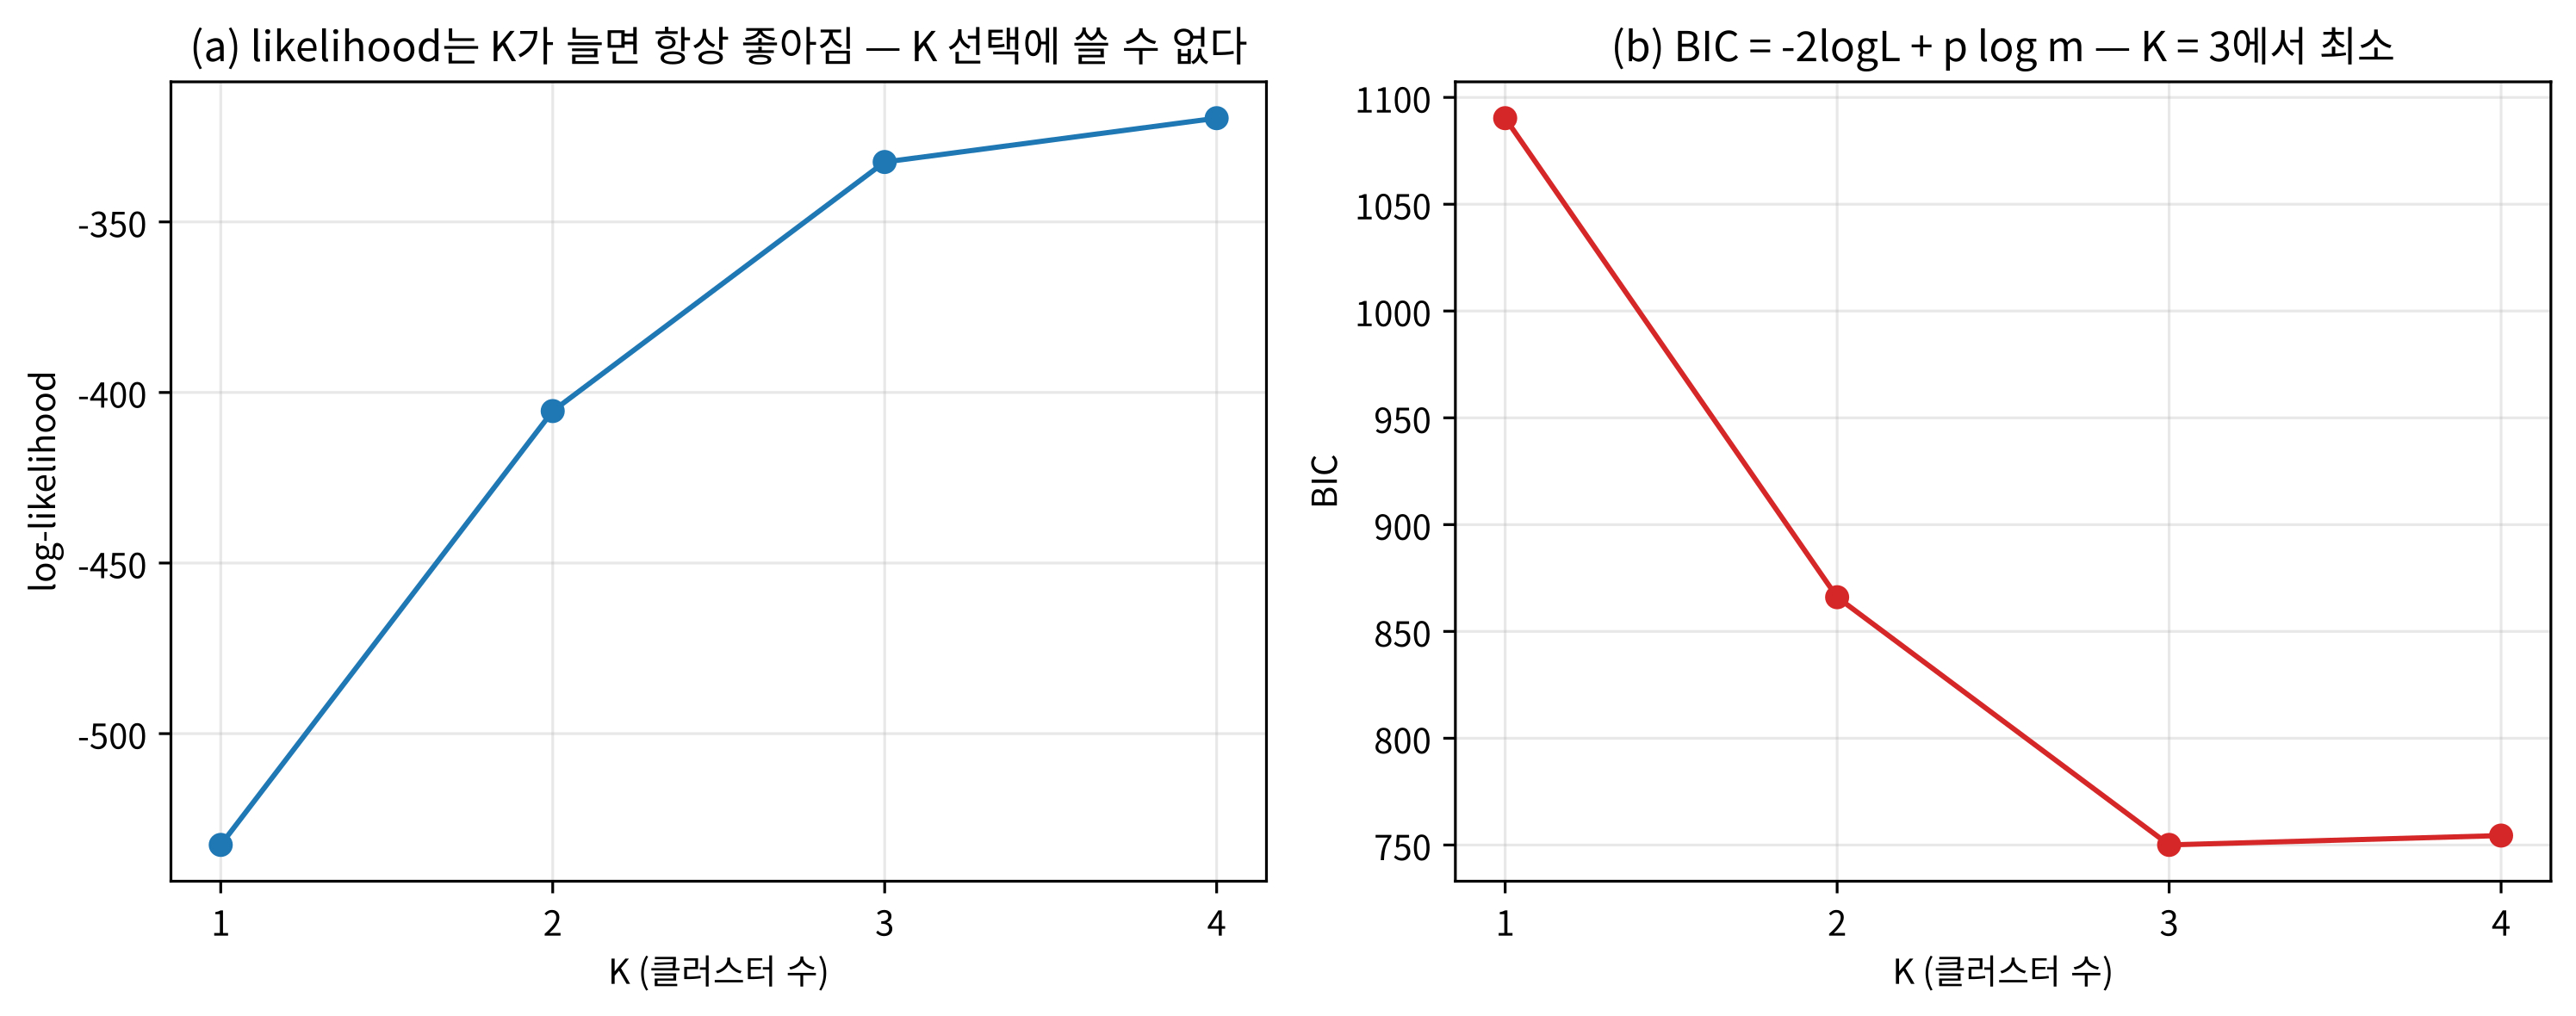
\includegraphics[width=0.92\linewidth]{ch15_gmm_bic.png}
    \end{column}
  \end{columns}
  \vskip0.3em
  $K=3\to4$: log-likelihood \textbf{동일}($-410.1$, 네 번째
  클러스터는 피팅을 안 높이고 기존 덩어리만 쪼갬)인데 \textbf{BIC
  벌점}($p$: 11$\to$15)이 판을 뒤집음. 엘보우가 그 꺾임을 \textbf{눈}
  으로 찾은 것을, BIC는 하나의 \textbf{숫자}로 내리는 원리 있는
  버전.
\end{frame}

\begin{frame}{같은 EM, 다른 데이터: LDA 개요}
  GMM을 생성 과정 관점에서 보면, ``데이터가 \textbf{어디서}
  만들어졌는가''(잠재변수 $z_i$ 한 줄기)를 모델링. 그런데
  데이터가 \textbf{점}으로만 만들어지는 것은 아니다:
  \textbf{문서}(뉴스·논문·리뷰)의 경우 ``이 문서가 \textbf{어떤
  주제로} 만들어졌는가''를 물으면, 잠재변수는 \textbf{$K$개
  주제의 혼합 비율} $\theta_d$($\sum_k \theta_{dk} = 1$)가
  된다.
  \vskip0.6em
  이 질문을 \textbf{같은 EM의 틀}로 푸는 것이
  \kb{LDA}(Latent Dirichlet Allocation, 잠재 디리클레 할당)
  --- 2003년 \kb{블레이(Blei)·응(Ng)·조던(Jordan)}.
  \begin{itemize}\small
    \item 이름의 \textbf{Dirichlet} = 사전분포의 이름,
      \textbf{Allocation} = ``할당'' --- \textbf{문서가 토픽에
      할당되고, 토픽이 단어에 할당}된다는 생성 과정
    \item ``\textbf{GMM의 ``점 $\to$ 클러스터''를 ``단어
      $\to$ 토픽''으로 바꾼 것}'' --- 같은 EM 계열의 고전
      확률모델
  \end{itemize}
\end{frame}

\begin{frame}{LDA의 생성 과정: GMM 골격 그대로}
  ``\textbf{주사위를 굴리고, 그 주사위 결과의 분포에서
  샘플링한다}''는 두 단계:
  \begin{enumerate}
    \item \kb{토픽 혼합 뽑기}: 문서 $d$의 토픽 혼합
      $\theta_d$를 \kb{디리클레 사전분포}
      $\text{Dir}(\alpha)$에서 뽑음 ($K$개 주제에 대한
      확률벡터 --- GMM의 혼합비율 $\pi$에 대응)
    \item \kb{단어 뽑기}: 문서의 \textbf{각 단어 위치} $n$마다,
      (i) 주사위 $\text{Categorical}(\theta_d)$로 토픽
      $z_{dn}$ 뽑고, (ii) 그 토픽의 \textbf{단어 분포}
      $\phi_{z_{dn}}$에서 단어 $w_{dn}$ 뽑음
  \end{enumerate}
  \vskip0.6em
  \begin{itemize}
    \item $\phi_k$ = ``\textbf{주제 $k$의 단어 프로필}'' ---
      '정치' 토픽이면 ``선거·정책·대통령'', '경제'면
      ``금리·물가·주식''이 높은 확률을 갖는 \textbf{어휘 크기
      만큼의} 확률벡터. $\phi_k$도 디리클레 사전
      $\text{Dir}(\beta)$에서 뽑힘
    \item $\alpha, \beta$ = ``문서가 주제를 어떻게
      \textbf{섞는지}'', ``토픽이 단어를 어떻게
      \textbf{섞는지}''에 대한 \textbf{사전적 믿음}을 담은
      하이퍼파라미터 --- 통상 \textbf{균일한 작은 값}
      (예: $\alpha = 50/K,\ \beta = 0.01$)
  \end{itemize}
  \vskip0.4em
  \begin{block}{켤레성의 선물}
    디리클레 분포는 단순히 ``확률벡터 위의 분포''가 아니라
    \textbf{다항분포의 켤레(conjugate) 분포}라
    \textbf{E-step과 M-step이 전부 닫힌 형태로 유지}
    --- GMM의 정규-감마 구조가 해준 것과 \textbf{정확히 같은
    역할}.
  \end{block}
\end{frame}

\begin{frame}{LDA의 E/M-step: GMM과의 대비}
  E/M-step은 ``\textbf{책임값이 무엇으로 바뀌는가}''만
  다를 뿐:
  \begin{itemize}\small
    \item \kb{E-step}: 문서 \textbf{각 단어 위치}의 \textbf{토픽
      사후확률} $\gamma_{dnk} = P(z_{dn} = k \mid w_d, \theta,
      \phi)$ --- GMM의 ``점 $i$가 \textbf{클러스터} $k$일
      확률''이 ``문서 $d$의 $n$번째 \textbf{단어}가 \textbf{토픽}
      $k$에서 왔을 확률''로 바뀜(관측 데이터가 점 대신 \textbf{단어})
    \item \kb{M-step}: 책임값으로 두 파라미터 갱신 ---
      $\theta_{dk} \propto \sum_n \gamma_{dnk}$(이 문서가
      토픽 $k$를 쓰는 비중), $\phi_{kw} \propto \sum_{d,n:\,
      w_{dn} = w} \gamma_{dnk}$(토픽 $k$에서 단어 $w$가
      나온 누적 책임) --- GMM의 ``책임값 \textbf{가중 평균}''과
      \textbf{동일한 구조}
  \end{itemize}
  \vskip0.6em
  엄밀히는 ``\textbf{완전한 EM}''이 아님 --- E-step이 각 단어
  위치의 토픽을 \textbf{독립}으로 근사하는 \textbf{변분
  추론}(mean-field 근사), 정석 명칭은 \textbf{변분 EM
  (VEM)}. ``계산 안 되는 E-step을 근사한다''는 수법은
  Ch.\,15.1절 \kb{VAE}가 \textbf{신경망}으로 하는 것의
  \textbf{가장 고전적인 예시} --- VAE가 신경망으로 근사하는
  것을, LDA는 ``\textbf{위치별 독립}''이라는 더 단순한 가정으로
  근사한 셈.
  \vskip0.4em
  \textbf{실전}: LDA 계열 토픽모델로 \textbf{뉴스 분류 ·
  의견 분석 · 문서 자동 요약}, 14.3절 문서 임베딩·RAG에서
  ``어떤 문서가 관련 있는가''를 판정하는 \textbf{보조 도구}.
\end{frame}

\begin{frame}{GMM vs LDA 한 표로}
  \scriptsize
  \begin{tabular}{@{}p{0.14\textwidth}p{0.36\textwidth}p{0.36\textwidth}@{}}
    \toprule
     & \textbf{GMM} & \textbf{LDA} \\
    \midrule
    관측 데이터 & 점 $x_i \in \mathbb{R}^d$ & 문서의 \textbf{단어}
               $w_{dn}$(이산) \\
    잠재변수 & 클러스터 라벨 $z_i$(1개/점) & 토픽 $z_{dn}$(1개/단어)
               + 혼합 $\theta_d$(1개/문서) \\
    ``덩어리''의 모양 & 정규분포 $\mathcal{N}(\mu_k, \Sigma_k)$ &
               \textbf{단어 분포} $\phi_k$(디리클레 사전 위) \\
    ``클러스터''의 의미 & 특징공간에서 \textbf{가까이 모인 점} &
               \textbf{자주 함께 나타나는 단어 패턴}(토픽) \\
    M-step 갱신 & $\mu_k, \Sigma_k, \pi_k$ & $\theta_d, \phi_k$ \\
    \bottomrule
  \end{tabular}
  \vskip1em
  \begin{block}{한 줄}
    ``클러스터''가 특징공간에서의 \textbf{기하학적 근접성}(GMM)이
    아니라 \textbf{단어 공출현의 통계적 패턴}(LDA)으로 바뀜 ---
    이것이 \textbf{같은 EM}의 두 가지 얼굴을 가질 수 있는
    이유. $K$ 선택 문제도 그대로 이어짐(토픽 수 선택도
    \textbf{BIC 계열 트레이드오프} --- 다만 우도를 닫힌 형태로
    계산할 수 없어 \textbf{변분 하한}을 기준으로 삼음).
  \end{block}
  \vskip0.6em
  {\footnotesize \textbf{이름 충돌 주의} --- 이 책에서 ``LDA''가
  \textbf{두 번} 등장한다. Ch.\,3.2의 \textbf{피셔 선형 판별}(Fisher's
  Linear Discriminant)도 LDA다 --- \textbf{서로 다른 문제를 푸는
  별개의 모델}이 나중에 \textbf{약자를 공유}한 것. \textbf{이 절의
  LDA} = 전부 \textbf{``잠재 디리클레 할당''}(Blei--Ng--Jordan,
  NIPS 2001 / JMLR 2003). \textbf{차원축소/분류의 LDA}는 3.2절의
  문맥에서만 등장.}
\end{frame}

\begin{frame}{자주 하는 실수 3가지}
  \small
  \begin{enumerate}
    \item \textbf{EM을 한 번만 돌려 믿기}(k-means 실수보다
      \textbf{더 위험}) --- k-means의 ``나쁜 초기화 $\to$
      나쁜 지역최적해''가 GMM에도 그대로 있지만, GMM은
      \textbf{분산까지 자유}라 실패의 모양이 다름: 무작위
      초기화 30회 중 여러 건이 \textbf{세 중심이 모두 데이터의
      중심 (2.98, 2.04)에 겹쳐서} 수렴하는 \textbf{퇴화된 해}
      --- 한 클러스터의 분산이 아주 작아져 ``가장 빽빽한 부분을
      $K$개의 작은 가우시안으로 쪼갠다''는 분할이
      \textbf{지역적으로는 우도 최대}가 되기 때문
      (log-likelihood $-749$ vs 진짜 구조 $-410$ ---
      \textbf{2.7배}나 나쁨). k-means의
      ``60회 중 실패''와 \textbf{같은 구조}의 문제인데, GMM은
      ``\textbf{분산이 붕괴}해 한두 점을 혼자 차지한다''는
      \textbf{추가 경로}까지 열려 있음. 대응책: \textbf{여러
      초기화}(\texttt{n\_init}) + \textbf{최종 우도로} 결과
      비교(\textbf{최대} 우도를 가진 결과 채택)
    \item \textbf{``likelihood가 가장 큰 $K$를 고른다''} ---
      $K = m$이 \textbf{항상} 이김(위 BIC 섹션).
      \textbf{BIC/AIC/교차검증}을 써야
    \item \textbf{책임값 0.4를 ``오류''로 읽기} ---
      클러스터가 겹치는 영역에서 $\gamma = (0.4, 0.6)$가
      나온 것은 모델이 \textbf{불확실성을 바르게 보고한
      것}이지 학습이 안 된 것이 아님. k-means로 같은 영역을
      색칠하면 \textbf{임의로 한쪽 색}이 붙어 ``확실히
      속한다''는 \textbf{거짓된 인상}을 줌 ---
      \textbf{soft assignment의 불확실성 정보}는
      (예: 경계점만 따로 골라 \textbf{인간이 재분류}하는)
      후속 작업에 실제로 유용
  \end{enumerate}
\end{frame}

\begin{frame}{자주 묻는 질문 (4.4)}
  \small
  \begin{itemize}
    \item \textbf{Q. EM이 항상 전역 최적해로 수렴하나요?}
      \textbf{아니} --- 매 반복마다 우도가 절대 \textbf{감소하지
      않음}(그래서 언젠가 수렴)은 보장되지만, 4.3절 k-means와
      마찬가지로 초기 파라미터에 따라 \textbf{지역 최적해}에
      갇힐 수 있음. 실전: \textbf{서로 다른 초기화로 여러 번
      돌려 가장 좋은 것을 채택}(k-means와 정확히 같은 대응책)
    \item \textbf{Q. GMM이 k-means보다 항상 더 좋은가?}
      \textbf{아니} --- GMM은 각 클러스터가 정규분포를 따른다는
      가정(Ch.\,3.2 GDA와 동일) + 부드러운 soft 할당 계산
      $\Rightarrow$ k-means보다 \textbf{계산 비용 더 듦}.
      클러스터가 \textbf{겹쳐 있거나 모양이 서로 다를} 가능성이
      있으면 GMM 유리, \textbf{뚜렷이 분리돼 있고 속도가
      중요}하면 k-means로 충분
    \item \textbf{Q. GMM의 E-step이 ``정확한'' 사후확률을 계산
      한다면, VAE는 왜 신경망으로 근사하나요?}
      GMM의 잠재변수 $z$는 \textbf{이산}이고 가능치가 $K$개
      뿐이라, 사후확률을 $K$개 항의 합으로 \textbf{정확히}
      계산 가능. VAE(15.1절)의 잠재변수는 \textbf{연속}
      벡터라 가능한 $z$가 \textbf{무한}하고, 사후확률의
      \textbf{적분이 계산 불가능}(intractable)
      $\Rightarrow$ ``계산 안 되는 E-step''을 \textbf{신경망}
      $q_\phi(z|x)$로 근사하고 M-step도 \textbf{역전파}로
      --- VAE는 정확히 이 필요에서 나온 \textbf{``EM의 약한
      근사 버전''}
    \item \textbf{Q. EM은 얼마나 빨리 수렴하나요?}
      통상 \textbf{선형(linear) 수렴} --- 수렴점 가까울수록
      오차가 ``고정된 비율''로 줄어들어 \textbf{마지막 몇 자리
      정밀도는 의외로 오래} 걸림. 실전: ``파라미터 변화가
      $\epsilon$ 미만''이나 ``likelihood 변화가 $\epsilon$
      미만'' 같은 \textbf{수렴 기준}. 고차원에선 $\Sigma_k$가
      \textbf{특이}(singular, 역행렬이 없는) 행렬에 \textbf{가깝게}
      수렴하기 쉬우니, 실전 라이브러리
      (\texttt{sklearn.mixture.GaussianMixture} 등)는
      (i) \textbf{대각 공분산}만 허용, (ii) 모든 클러스터
      \textbf{같은 공분산}, (iii) $\Sigma_k + \epsilon I$ 같은
      \textbf{정규화} 옵션 제공
    \item \textbf{Q. ``생성 모델''이라면서 어떻게 데이터를
      \emph{만들어}냅니까?}
      학습이 끝나면 \textbf{완전한} 데이터 생성 절차
      $p(z) \to p(x|z)$를 가짐 --- 새 점: (1) 주사위 $\pi$로
      $z$ 뽑고, (2) 그 $z = k$의 $\mathcal{N}(\mu_k, \Sigma_k)$
      에서 $x$ 샘플링. 이 ``생성'' 능력이 Ch.\,15(VAE가
      $z \sim \mathcal{N}(0, I)$에서, GAN이 \textbf{노이즈}
     에서)의 ``데이터 생성''과 \textbf{정확히 같은 질문}의
      가장 단순한 버전
  \end{itemize}
\end{frame}

\begin{frame}{실습으로 연결하기 (4.4)}
  노트북 \texttt{chapter04\_4\_gmm\_em.ipynb}은
  numpy/matplotlib만으로 본문 코드를 그대로 실행:
  \begin{enumerate}\small
    \item 책의 \texttt{em\_step}을 \textbf{6개 데이터}에 돌려
      \textbf{수렴 과정 추적}(1차원) --- 앞의
      $-15.56 \to -6.05 \to -6.05$ 표
    \item 3개 블롭 2차원 데이터에서 \textbf{2D GMM}을 EM으로
      학습, \textbf{등고선 + 책임값 기반 색칠}로 시각화
    \item \textbf{무작위 초기화 30회} 돌려
      \textbf{지역 최적해/분산 붕괴 실패 사례}를 실제로 만든
      뒤 좋은 초기화와 log-likelihood로 비교
    \item $K = 1\sim4$의 \textbf{BIC 곡선}을 그려
      $K$ 선택 확인(최소 $K=3$)
  \end{enumerate}
  \vskip0.6em
  {\footnotesize 본문의 특정 숫자(실패 횟수, BIC 값 등)는
  재현을 목표로 하지는 않으며, 같은 \textbf{``현상''}이 실제로
  일어나는지 확인하는 것.}
\end{frame}

% ===== wrap-up =====
\begin{frame}{이번 주차 정리}
  \small
  \begin{enumerate}
    \item \kb{4.1 kNN} --- 게으른·비모수 방법, 예측 비용
      $O(m\cdot d)$. \textbf{정규화 빼먹으면} 0.556$\to$1.000
      반전의 실수. $k$를 키우며 \textbf{편향-분산} 트레이드오프:
      톱니바퀴(과적합) $\to$ 직선(과소적합). $k=1$ 결정경계 =
      \textbf{보로노이 다이어그램}.
    \item \kb{4.2 차원의 저주} --- 부피 $0.5^n$ 증발,
      $p^{1/n}$ 스케일, \textbf{이웃이 동거리에}
      ($11^{1/n}\to1$). junk 축 50개 $\to$ 정확도
      0.867$\to$\textbf{0.507}. $k$는 \textbf{검증셋}으로
      고르고, ``훈련 정확도로 고르면 \textbf{항상 $k=1$}''
      함정.
    \item \kb{4.3 k-means} --- ``할당$\to$갱신''이 \textbf{SSE를
      단조감소}시켜 수렴(단, \textbf{어디로}는 보장 안 됨).
      \textbf{엘보우}로 $k$ 선택, \textbf{k-means++}
      ($D(x)^2$-비례, $O(\log k)$ 보장) + \texttt{n\_init}.
      경계가 \textbf{항상 직선(볼록)}이라는 \textbf{구조적
      한계}. 로이드(1957)·매퀸(1967) 동시 발견.
    \item \kb{4.4 GMM/EM} --- 하드 $\to$ \textbf{소프트
      할당}. 라벨·파라미터 ``둘 다 모른다''는 순환을
      E-step(책임값) $\to$ M-step(가중 평균)으로 반복.
      \textbf{옌센 부등식 4줄} = ``우도가 절대 줄지 않는다''.
      $\Sigma_k$가 \textbf{타원형·기울어진} 클러스터. $K$는
      \textbf{BIC}로, \textbf{분산 붕괴} 퇴화 해 주의.
      \textbf{LDA} = GMM의 ``점$\to$클러스터''를
      ``단어$\to$토픽''으로.
  \end{enumerate}
  \vskip0.8em
  \begin{block}{다음 주차 --- Chapter 5. SVM과 커널}
    kNN의 결정경계는 ``이웃 순위''에 따라 결정되는
    \textbf{국소적} 경계(보로노이). 다음 장은 반대로
    ``무수히 많은 경계선 중 \textbf{어떤 것이 새 데이터에 가장
    안전한가}''라는 \textbf{전역적·기하학적} 질문을 던지며,
    그 답으로 \textbf{마진 최대화(SVM)}(Cortes \& Vapnik 1995)
    와 \textbf{커널 트릭}을 소개한다.
  \end{block}
\end{frame}

\end{document}
